\documentclass[11pt]{elegantbook}
\definecolor{structurecolor}{RGB}{40,58,129}
\linespread{1.6}
\setlength{\footskip}{20pt}
\setlength{\parindent}{0pt}
\newcommand{\argmax}{\operatornamewithlimits{argmax}}
\newcommand{\argmin}{\operatornamewithlimits{argmin}}
\elegantnewtheorem{proof}{Proof}{}{Proof}
\elegantnewtheorem{claim}{Claim}{prostyle}{Claim}
\DeclareMathOperator{\col}{col}
\title{Notes of Probability}
\author{Wenxiao Yang}
\institute{Department of Mathematics, University of Illinois at Urbana-Champaign}
\date{2022}
\setcounter{tocdepth}{2}
\extrainfo{All models are wrong, but some are useful.}

\cover{cover.jpg}

% modify the color in the middle of titlepage
\definecolor{customcolor}{RGB}{32,178,170}
\colorlet{coverlinecolor}{customcolor}
\usepackage{cprotect}

\addbibresource[location=local]{reference.bib} % bib

\begin{document}
\maketitle

\frontmatter
\tableofcontents

\mainmatter

\chapter{Distribution}

\section{Discrete}
\subsection{Bernoulli Distribution -- $\operatorname{Bernoulli}(\pi)$: an event happens with probability $\pi$}
Assume $n$ independent binary (taking values $0$ or $1$) observations arising from independent and identical trials: $y_{1}, y_{2}, \ldots, y_{n}$ such that: $P\left(Y_{i}=1\right)=\pi$ and $P\left(Y_{i}=0\right)=1-\pi$.

Random variables $Y_{i}$ are normally called \textbf{Bernoulli} trials, $Y_{i} \sim \operatorname{Bernoulli}(\pi)$. $$\mathbb{E}(Y_i)=\pi,Var(Y_i)=\pi(1-\pi)$$

\subsection{Binomial distribution -- $bin(n,\pi)$: $n$ independent Bernoulli distributions}
The random variable $Y=\sum_{i=1}^{n} Y_{i}$ has the Binomial distribution with index $n$ and parameter $\pi$ denoted as $Y \sim \operatorname{bin}(n, \pi)$.
Mass probability function for $Y$ :
$$
P(y)=\left(\begin{array}{l}
n \\
y
\end{array}\right) \pi^{y}(1-\pi)^{n-y}
$$
with $\left(\begin{array}{l}n \\ y\end{array}\right)=\frac{n !}{y !(n-y) !}$ and $y=0,1,2, \ldots, n$
\begin{enumerate}[(1)]
    \item Mean and Variance:
    $\mathbb{E}(Y)=\mu=n \pi,\operatorname{Var}(Y)=\sigma^{2}=n \pi(1-\pi)$
    \item Skewness: $\mathbb{E}\frac{(Y-\mu)^{3}}{\sigma^{3}}=\frac{1-2 \pi}{\sqrt{n \pi(1-\pi)}}$
    \item If the independence assumption is violated, the Binomial distribution does not apply.
    \item Normal approximation:$\frac{Y-n \pi}{\sqrt{n \pi(1-\pi)}} \stackrel{d}{\longrightarrow} N(0,1),\quad {n \rightarrow \infty}$.
\end{enumerate}

\subsection{Multinomial Distribution}
Assume $n$ independent trials have outcomes in $c > 2$ categories. Let $y_{ij} = 1$ if trial $i$ has outcome in category $j$; otherwise $y_{ij} = 0$. For example, if $c = 5$, a possible outcome of a trail is $(0, 1, 0, 0, 0)$. The binary vector $\vec{y}_i = (y_{i1}, y_{i2}, . . . , y_{ic})$ represents a \underline{multinomial} trial.

Note that $\sum_{j}y_{ij}=1$ whereas $\sum_{i}y_{ij}=n_j$ is the number of outcomes for category $j$. Also note that $y_{ic}$ is redundant because it is dependent on the remaining outcomes: $y_{ic} = 1 - \sum_{j=1}^{c-1} y_{ij}$.

The vector of counts $(n_1,n_2,...,n_c)$ has a multinomial distribution, with mass probability function:
\begin{equation}
    \begin{aligned}
        p(n_1,n_2,...,n_{c-1})=\frac{n!}{n_1!n_2!...n_c!}\pi_1^{n_1}\pi_2^{n_2}...\pi_c^{n_c}
    \end{aligned}
    \nonumber
\end{equation}
where $\pi_j=\textnormal{Pr}(Y_{ij}=1)$
\begin{enumerate}
    \item Please note that the marginal distribution of each $n_j$ is a binomial distribution.
    \item The binomial distribution is a special case of the multinomial distribution when $c = 2$.
    \item $\mathbb{E}(n_j)=n\pi_j$, $\textnormal{Var}(n_j)=n\pi_j(1-\pi_j)$, $\textnormal{Cov}(n_j,n_k)=-n\pi_j\pi_k$.
    \item Entries of correlation matrix: $$\rho(n_j,n_j)=1,\forall j;\ \rho(n_j,n_k)=\frac{\textnormal{Cov}(n_j,n_k)}{\sqrt{\textnormal{Var}(n_j)\textnormal{Var}(n_k)}}=-\sqrt{\frac{\pi_j\pi_k}{(1-\pi_j)(1-\pi_k)}},\forall j\neq k$$
\end{enumerate}




\subsection{Poisson Distribution -- $Pois(\lambda)$: an event happens $k$ times within unit time}
$\lambda$: frequency of the event, i.e., the average number of event happens within unit time.
$$\Pr(X{=}k)= \frac{\lambda^k e^{-\lambda}}{k!},\ k=0,1,2,3...$$
$$E(X)=Var(X)=\lambda$$
\begin{center}\begin{figure}[htbp]
    \centering
    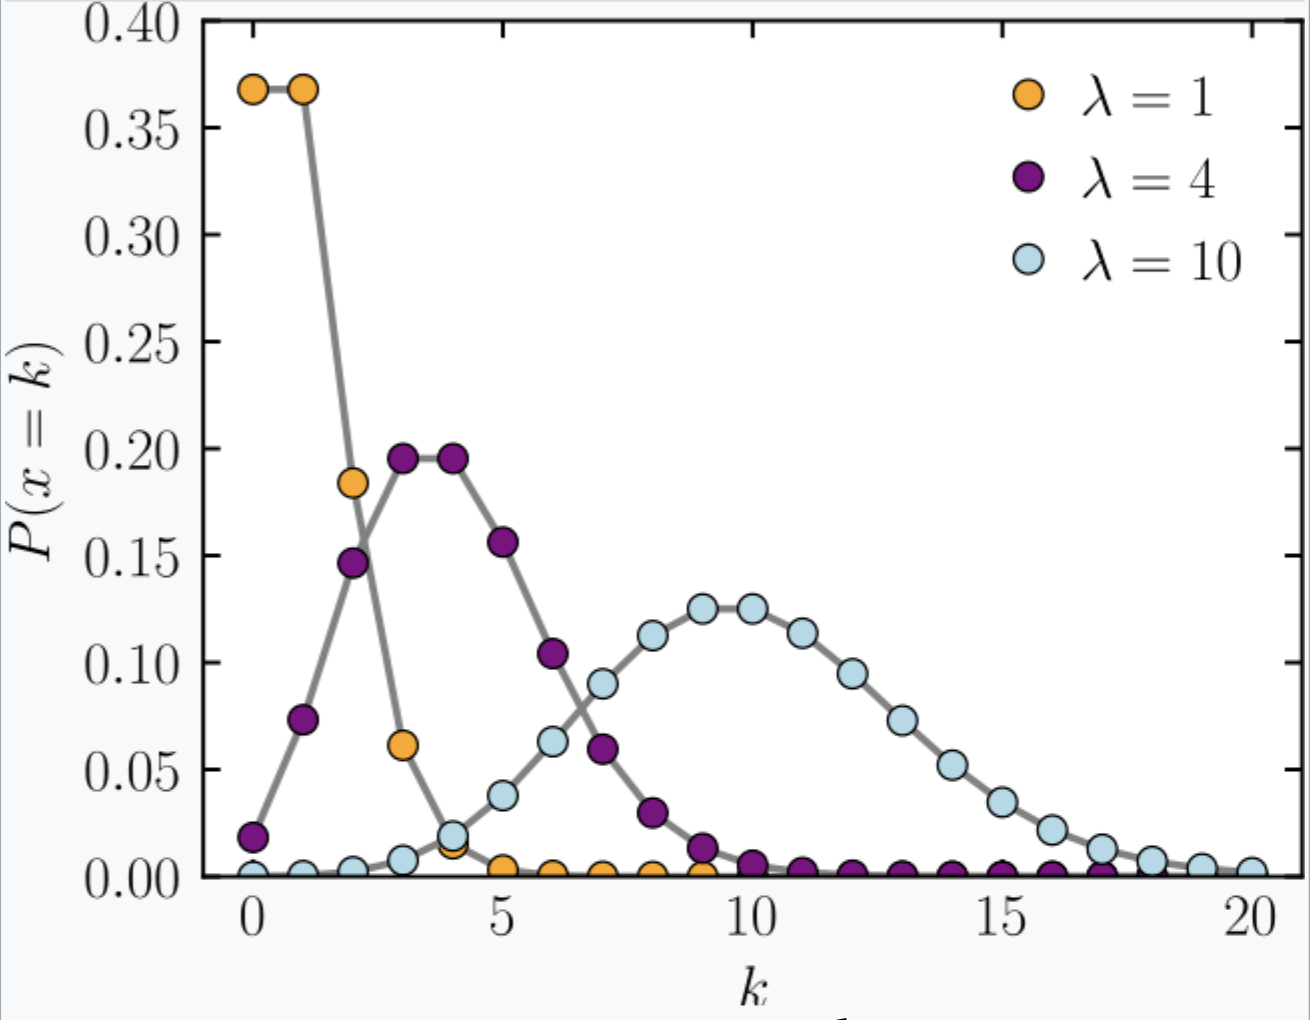
\includegraphics[scale=0.2]{Poisson Distribution graph.png}
    \caption{The Poisson pmf is unimodal with mode equal to the integer part of $\lambda$.}
\end{figure}\end{center}
\vspace{-1cm}
Its skewness (measure of the asymmetry of the probability distribution) is: $\mathbb{E}\frac{(X-\mu)^3}{\sigma^3}=\frac{1}{\sqrt{\lambda}}$. That is the higher the $\lambda$ is, the less skew the distribution is.

\subsubsection*{Derivation process (an approximation to the binomial distribution when $n$ is large and $\pi$ is small, such that $\mu=n\pi$.)}
Consider a unit time (the unit is divided into $n$ equal subparts, $n \rightarrow \infty$), there is an event may occur with every subpart, the number of the event happens should follow binomial distribution $B(n,p)$. where $n \rightarrow \infty, p \rightarrow 0$; $\lambda=n\cdot p$ is the expected number of events in this period of time.

The probability the number of the event happens:
\begin{equation}
    \begin{aligned}
        \Pr(X=k)&=\lim_{n \rightarrow\infty} \binom{n}{k} (\frac{\lambda}{n})^k(1-\frac{\lambda}{n})^{n-k}\\
        &=\lim_{n \rightarrow\infty} \frac{n!}{(n-k)!k!} (\frac{\lambda}{n})^k(1-\frac{\lambda}{n})^{n}(1-\frac{\lambda}{n})^{-k}\\
        &=\lim_{n \rightarrow\infty}\frac{n!}{(n-k)!k!} (\frac{\lambda}{n})^k e^{-\lambda}\\
        &=\frac{\lambda^k e^{-\lambda}}{k!}\lim_{n \rightarrow\infty}\frac{n!}{(n-k)!n^k}\\
        &=\frac{\lambda^k e^{-\lambda}}{k!}\lim_{n \rightarrow\infty}
        \frac{n}{n}\frac{n-1}{n}\cdots \frac{n-k+1}{n}\\
        &=\frac{\lambda^k e^{-\lambda}}{k!}
    \end{aligned}
    \nonumber
\end{equation}

\subsubsection*{Sums of independent Poisson random variables are Poisson random variables}
$X\sim Pois(\lambda_1), Y\sim Pois(\lambda_2)$ are two independent Poisson random variables, then $Z=X+Y$ also follow Poisson distribution, and the paramenter is the sum of $X$'s and $Y$'s
\begin{equation}
    \begin{aligned}
        Z\sim Pois(\lambda_1+\lambda_2)
    \end{aligned}
    \nonumber
\end{equation}
Then, $$Z=X_1+X_2+\cdots+X_n\sim Pois(\lambda_1+\lambda_2+\cdots+\lambda_n)$$

\subsection{Connection between Poisson and multinomial distribution}
Consider a sum of independent Poisson random variables $Y_i$ with parameters $\lambda_i$. $\sum_i Y_i$ has a Poisson distribution with parameter $\lambda=\sum_i \lambda_i$. If $\sum_i Y_i=n$ and $n$ is fixed, the random variables $Y_i\mid n$ are no longer independent nor have a Poisson distribution.

For a $c$ number of Poisson random variables, we can calculate the joint probability distribution of a set of counts $\{n_i\}$ conditioned on $\sum_i Y_i=n$ as:
\begin{equation}
    \begin{aligned}
        P(Y_1 = n_1,Y_2 = n_2,...,Y_c = n_c\mid \sum_i Y_i=n) &=\frac{P(Y_1 = n_1,Y_2 = n_2,...,Y_c = n_c)}{P(\sum_i Y_i=n)}\\
        &=\frac{\prod_{i=1}^c \frac{e^{-\lambda_i} \lambda_i^{n_i}}{n_i !}}{\frac{e^{-\sum_{i}\lambda_i} (\sum_i\lambda_i)^{n}}{n !}}=\frac{n!}{n_1!n_2!...n_c!}\pi_1^{n_1}\pi_2^{n_2}...\pi_c^{n_c}
    \end{aligned}
    \nonumber
\end{equation}
where $\pi_i=\frac{\mu_i}{\sum_i\mu_i}$. This results in a multinomial $(n,\{\pi_i\})$ distribution.

\subsection{Geometric distribution: $P(X=k)=(1-p)^{k-1}p$}
The geometric distribution gives the probability that the first occurrence of success requires $k$ independent trials, each with success probability $p$. It is a discrete form of exponential distribution.
$$P(X=k)=(1-p)^{k-1}p,\ P(X\leq k)=1-(1-p)^k$$
\begin{equation}
    \begin{aligned}
        \mathbb{E}(X)=\frac{1}{p},\ Var(X)=\frac{1-p}{p^2}
    \end{aligned}
    \nonumber
\end{equation}

\section{Continuous}
\subsection{Exponential distribution $Exp(\lambda)$: interval between to independent identical event / the first time a event happened}
$\lambda$: frequency of the event.

$X$ follows exponential distribution with parameter $\lambda$ or $\beta$:
$${\displaystyle X\sim {\text{Exp}}(\lambda )} \text{ or } {\displaystyle X\sim {\text{Exp}}(\beta )}$$
They are equivlanet, the only difference is $\beta=\frac{1}{\lambda}$.
$${f(x;{\lambda})=\left\{{\begin{matrix}{\lambda }e^{-{\lambda }x}&x\geq 0\\0&\;x<0.\end{matrix}}\right.}$$
$${f(x;{\beta})=\left\{{\begin{matrix}{\frac{1}{\beta} }e^{-{\frac{1}{\beta} }x}&x\geq 0\\0&\;x<0.\end{matrix}}\right.}$$
c.d.f is:
$${F(x;{\lambda})=\left\{{\begin{matrix}{1-}e^{-{\lambda }x}&x\geq 0\\0&\;x<0.\end{matrix}}\right.}$$
Note that $\lambda > 0$ is the frequcy of the occurance of the event; $\beta>0$ is the probability of the event happens in each second. The range of exponential distribution is $[0,\infty)$.

$$\mathbb{E}(X)=\frac{1}{\lambda};\ Var(X)=\frac{1}{\lambda^2}$$
Memorylessness: ${\displaystyle \Pr \left(T>s+t\mid T>s\right)=\Pr(T>t)}$
\begin{equation}
    \begin{aligned}
        \Pr (T>s+t\mid T>s)&=\frac{\Pr(T>s+t\text{ and }T>s)}{\Pr(T>s)}\\
        &=\frac{\Pr(T>s+t)}{\Pr(T>s)}\\
        &=\frac{e^{-\lambda(s+t)}}{e^{-\lambda s}}\\
        &=e^{-\lambda t}\\
        &=\Pr (T>t)
    \end{aligned}
    \nonumber
\end{equation}

\subsection*{Derivation process:}

Consider a unit time (the unit is divided into $n$ equal subparts, $n \rightarrow \infty$), there is an event may occur with every subpart, the number of the event happens should follow binomial distribution $B(n,p)$. where $n \rightarrow \infty, p \rightarrow 0$; $\lambda=n\cdot p$ is the expected number of events in this period of time. (the same as Poisson)\\
CDF:
\begin{equation}
    \begin{aligned}
        1-F(x;\lambda)=\lim_{n \rightarrow \infty}(1-\frac{\lambda}{n})^{nx}=e^{-\lambda x}
        \Rightarrow F(x;\lambda)=1-e^{-\lambda x}
    \end{aligned}
    \nonumber
\end{equation}
PDF:
\begin{equation}
    \begin{aligned}
        f(x;\lambda)=\frac{\partial F(x;\lambda)}{\partial x}=\lambda e^{-\lambda x}
    \end{aligned}
    \nonumber
\end{equation}

\subsection{Gaussian/Normal Distribution}
$N(\mu,\sigma^2)$. p.d.f. ${\displaystyle f(x)={\frac {1}{\sigma {\sqrt {2\pi }}}}e^{-{\frac {1}{2}}\left({\frac {x-\mu }{\sigma }}\right)^{2}}}$
\begin{theorem}
Suppose $X\sim N(\mu_1,\sigma_1^2)$ and $Y\sim N(\mu_2,\sigma_2^2)$ are independent, then $X+Y\sim N(\mu_1+\mu_2,\sigma_1^2+\sigma^2)$.
\end{theorem}
\begin{proof}
The MGF of $X$ is
\begin{equation}
    \begin{aligned}
        M_X(t)=\mathbb{E}e^{tx}&=\int_{-\infty}^{\infty}e^{tx}\frac{1}{\sqrt{2\pi}\sigma_1}e^{-\frac{(x-\mu_1)^2}{2\sigma_1^2}}dx\\
        &=\int_{-\infty}^{\infty}\frac{1}{\sqrt{2\pi}\sigma_1}e^{-\frac{x^2-2(\mu_1+\sigma_1^2t)x+\mu_1^2}{2\sigma_1^2}}dx\\
        &=e^{\frac{\sigma_1^4t^2+2\mu_1\sigma^2t}{2\sigma_1^2}}\int_{-\infty}^{\infty}\frac{1}{\sqrt{2\pi}\sigma_1}e^{-\frac{(x-(\mu_1+\sigma_1^2t))^2}{2\sigma_1^2}}dx\\
        &=e^{t\mu_1+\frac{1}{2}\sigma_1^2t^2}
    \end{aligned}
    \nonumber
\end{equation}
Then, the MGF of $X+Y$ is
\begin{equation}
    \begin{aligned}
        M_{X+Y}(t)=\mathbb{E}e^{t(X+Y)}=\mathbb{E}e^{tX}\mathbb{E}e^{tY}=e^{t(\mu_1+\mu_2)+\frac{1}{2}(\sigma_1^2+\sigma_2^2)t^2}=M_{Z}(t)
    \end{aligned}
    \nonumber
\end{equation}
where $Z\sim N(\mu_1+\mu_2,\sigma_1^2+\sigma^2)$
\end{proof}

\subsection{Multivariate/Joint Gaussian/Normal Distribution (MVN)}
A $k$-dimensional random vector $(X_1,X_2,...,X_k)^T=\mathbf{X}\sim N(\mu,\Sigma)$.

p.d.f. $${\displaystyle f_{\mathbf {X} }(x_{1},\ldots ,x_{k})={\frac {\exp \left(-{\frac {1}{2}}({\mathbf {x} }-{\boldsymbol {\mu }})^{\mathrm {T} }{\boldsymbol {\Sigma }}^{-1}({\mathbf {x} }-{\boldsymbol {\mu }})\right)}{\sqrt {(2\pi )^{k}|{\boldsymbol {\Sigma }}|}}}}$$

A random vector is said to be $k$-variate normally distributed if every linear combination of its $k$ components has a univariate normal distribution.
\begin{enumerate}[(1)]
    \item $\mu$ is a $k$-dimensional \textbf{mean vector}: $$\mu=\mathbb{E}[\mathbf{X}]=(\mathbb{E}[X_1],\mathbb{E}[X_2],...,\mathbb{E}[X_k])^T$$
    \item $\Sigma$ is a $k\times k$ \textbf{covariance matrix}$${\displaystyle \Sigma _{i,j}=\operatorname {E} [(X_{i}-\mu _{i})(X_{j}-\mu _{j})]=\operatorname {Cov} [X_{i},X_{j}]}$$
    \item The inverse of $\Sigma$, ${\boldsymbol {Q}}={\Sigma }^{-1}$ is \textbf{precision matrix}.
\end{enumerate}
\begin{theorem}
    MVN distribution is completely specified by knowing $\mu$, $\Sigma$.
\end{theorem}
\begin{proof}
MGF: $M_X(t_1,t_2,...,t_k)=\mathbb{E}e^{\sum_{i=1}^k t_ix_i}$

Since any linear combination of $X$ is also normal distribution, $\Omega=\sum_{i=1}^k t_ix_i$ follows normal distribution.
$$M_X(t_1,t_2,...,t_k)=\mathbb{E}e^\Omega=e^{\mathbb{E}(\Omega)+\frac{1}{2}Var(\Omega)}=e^{\sum_{i=1}^kt_i \mathbb{E}(x_i)+\frac{1}{2}Var(\sum_{i=1}^k t_ix_i)}$$
\end{proof}

Generally, "independence" is a \textbf{stronger} condition than "$0$ correlation" ($Cov=0$).
\begin{theorem}
    For \textbf{MVN}, "independence" is \textbf{equivalent} to "$0$ correlation"
\end{theorem}
\begin{proof}
As we show $M_X(t_1,t_2,...,t_k)=e^{\sum_{i=1}^kt_i \mathbb{E}(x_i)+\frac{1}{2}Var(\sum_{i=1}^k t_ix_i)}$. If $Cov(x_i,x_j)=0,\forall i,j\in S$,
\begin{equation}
    \begin{aligned}
        M_X(t_1,t_2,...,t_k)&=e^{\sum_{i=1}^kt_i \mathbb{E}(x_i)+\frac{1}{2}Var(\sum_{i=1}^k t_ix_i)}\\
        &=e^{\sum_{i=1}^it_ki \mathbb{E}(x_i)+\frac{1}{2}\sum_{i=1}^it_i^2Var(x_i)}\\
        &=\prod_{i=1}^ke^{t_i\mathbb{E}(x_i)+\frac{1}{2}t_i^2Var(x_i)}\\
        &=\prod_{i=1}^kM_{x_i}(t_i)
    \end{aligned}
    \nonumber
\end{equation}
\end{proof}

\begin{theorem}
    Independent $X=[X_1,X_2,...,X_n]\sim$ MVN and $Y=[Y_1,Y_2,...,Y_m]\sim$ MVN, then $W=[X_1,X_2,...,X_n,Y_1,Y_2,...,Y_m]\sim$ MVN.
\end{theorem}

\begin{theorem}
    Independent $X=[X_1,X_2,...,X_n]\sim N(\mu_1,\Sigma_1)$ and $Y=[Y_1,Y_2,...,Y_n]\sim N(\mu_2,\Sigma_2)$, then $X+Y\sim N(\mu_1+\mu_2,\Sigma_1+\Sigma_2)$.
\end{theorem}














\section{Poisson process: A sequence of arrivals in continuous time with rate $\lambda$}
\subsection{Definition}
$N(t)\sim Pois(\lambda t)$: Number of arrivals in length $t$ follows Poisson distribution
\begin{equation}
    \begin{aligned}
        N(t)\sim Pois(\lambda t)\\
        \Pr(N(t)=k)=\frac{(\lambda t)^k e^{-\lambda t}}{k!}
    \end{aligned}
    \nonumber
\end{equation}
The number of arrivals in disjoint time intervals are independent.
\subsection{$T_j$: time of $j^{th}$ arrival}
$T_1>t$ is same as $N(t)=0$: $P(T_1>t)=P(N(t)=0)=e^{-\lambda t}$\\
$\Rightarrow T_1\sim Expo(\lambda) \Rightarrow T_j-T_{j-1}\sim Expo(\lambda); T_j\sim Gamma(j,\lambda)$

\subsection{Theorem (Conditional counts): $N(t_1)|N(t_2)=n\sim Bin(n,\frac{t_1}{t_2})$}
(We can interpret the theorem as: $n$ points distribute uniformly in $(0,t_2]$, so the probability a point loctae within $(0,t_1]$ is $\frac{t_1}{t_2}$)

\chapter{Basis}
\section{Covariance and Variance}
\begin{enumerate}[(1)]
    \item $\sigma_{XY}=Cov(X,Y)=\mathbb{E}\left[(X-\mathbb{E}X)(Y-\mathbb{E}Y)\right]=\mathbb{E}(XY)-\mathbb{E}X\mathbb{E}Y$
    \item $Cov(aX+b,Y)=aCov(X,Y)$
    \item $Cov(X+Y,W)=Cov(X,W)+Cov(Y,W)$
    \item $Cov(aX+bY,cX+dY)=ac\ {Var}(X)+(ad+bc)Cov(X,Y)+bd\ {Var}(Y)$
    \item $Var(aX+bY)=a^2\ {Var}(X)+2ab\ Cov(X,Y)+b^2\ {Var}(Y)$
\end{enumerate}
\section{Conditional Expectation and Variance}
\begin{enumerate}[(1)]
    \item Conditional variance: $$Var(Y|X=x)=\mathbb{E}\left((Y-\mathbb{E}(Y|X=x))^2|X=x\right)
    =\mathbb{E}(Y^2|X=x)-(\mathbb{E}(Y|X=x))^2$$
    \item \textbf{Law of Total Expectation:} $$\mathbb{E}(Y)=\sum_{i=1}^n \mathbb{E}(Y|A_i)P(A_i)$$
    \item \textbf{Law of Iterated Expectation (Adam's Law):}
    $$\mathbb{E}\left[\mathbb{E}(Y|X)\right]=\mathbb{E}(Y)$$
    \item \textbf{Adam's Law with extra conditioning:} $$\mathbb{E}\left(\mathbb{E}(Y|X,Z)|Z\right)=\mathbb{E}(Y|Z)$$
    \item \textbf{Law of Total Variance:}$$Var(Y)=\mathbb{E}(Var(Y|X))+Var(\mathbb{E}(Y|X))$$
\end{enumerate}

\section{Gambler's Ruin}
Suppose a gambler at each round either wins a dollar or loses a dollar with probability $\frac{1}{2}$ each. Suppose the gambler starts at $k$ dollars. He stops when either he reaches his goal of $N$ dollars or he goes bankrupt and loses all his money.

Let $A$ be the event that the gambler is ruined.
\begin{equation}
    \begin{aligned}
        P(A|x=k)=\frac{1}{2}P(A|x=k-1)+\frac{1}{2}P(A|x=k+1)\\
        \Rightarrow p_k-p_{k-1}=p_{k+1}-p_k
    \end{aligned}
    \nonumber
\end{equation}
According to the setting, $p_0=1,p_N=0$, then $p_k=\frac{N-k}{N}$.

\section{Moment Generating Function (MGF)}
\begin{definition}[Moment Generating Function (MGF)]
    Let $X$ be a random variable. The moment generating function (mgf) of $X$, denoted by $M_X(t)$:
    \begin{equation}
        \begin{aligned}
            M_X(t)&=\mathbb{E}[e^{tX}]\\&=\mathbb{E}\left[1+tX+\frac{(tX)^2}{2!}+\frac{(tX)^3}{3!}+\cdots\right]=\sum_{n=0}^\infty\frac{\mathbb{E}[X^n]t^n}{n!}
        \end{aligned}
        \nonumber
    \end{equation}
\end{definition}
Let $X$ be a random variable. The moment generating function (mgf) of $X$, denoted by $M_X(t)$:
\begin{equation}
    \begin{aligned}
        \underline{M_X(t)=\mathbb{E}[e^{tX}]}=\mathbb{E}\left[1+tX+\frac{(tX)^2}{2!}+\frac{(tX)^3}{3!}+\cdots\right]=\sum_{n=0}^\infty\frac{\mathbb{E}[X^n]t^n}{n!}
    \end{aligned}
    \nonumber
\end{equation}
We can find $\frac{\partial M_X(t)}{\partial t}= \mathbb{E}\left[Xe^{tX}\right]$, then $\frac{\partial M_X(0)}{\partial t}= \mathbb{E}\left[X\right]$. More generally, we can find that $$\frac{\partial^n M_X(0)}{\partial t^n}= \mathbb{E}\left[X^n\right],n=1,2,...$$
\subsection*{Why MGF is useful?}
\begin{enumerate}[(1)]
    \item If $X,Y$ are independent, then $$M_{X+Y}(t)=\mathbb{E}[e^{(X+Y)t}]=\mathbb{E}[e^tX]\mathbb{E}[e^tY]=M_X(t)M_Y(t)$$
    \item Unique random variable (RV) $\Leftrightarrow$ unique MGF
\end{enumerate}

\section{Inequality}
\subsection{Cauchy-Schwarz inequality: $|\mathbb{E}XY|\leq \sqrt{\mathbb{E}X^2\cdot \mathbb{E}Y^2}$}
For any r.vs. $X$ and $Y$ with finite variance: $|\mathbb{E}XY|\leq \sqrt{\mathbb{E}X^2\cdot \mathbb{E}Y^2}$
\begin{example}[Second Moment Method]
$X$ is a non-negative r.v. We want to find an \underline{upper bound} on $P(X=0)$.
\end{example}
Because $X$ is non-negative, $X=X\cdot \textbf{I}_{X>0}=\left\{\begin{matrix}
    X,&X>0\\
    0,&X=0
\end{matrix}\right.$. Hence,
\begin{equation}
    \begin{aligned}
        \mathbb{E}X= \mathbb{E}X\cdot \textbf{I}_{X>0}\leq \sqrt{\mathbb{E} X^2\cdot \textbf{I}^2_{X>0}}=\sqrt{\mathbb{E}X^2}\sqrt{P(X>0)}\\
        \Rightarrow P(X>0)\geq\frac{(\mathbb{E}X)^2}{\mathbb{E}X^2} \Rightarrow P(X=0)=1-P(X>0)\leq \frac{Var(X)}{\mathbb{E}X^2}
    \end{aligned}
    \nonumber
\end{equation}

\subsection{Jensen's Inequality: convex $g$ $\Rightarrow$ $\mathbb{E}(g(X))\geq g(\mathbb{E}(X))$}
If $g$ is convex $\mathbb{E}(g(X))\geq g(\mathbb{E}X)$; If $g$ is concave $\mathbb{E}(g(X))\leq g(\mathbb{E}X)$.

\subsection{Markov's Inequality: $P(|X|\geq a)\leq \frac{\mathbb{E}|X|}{a}$}
For any r.v. $X$ and a constant $a>0$. $P(|X|\geq a)\leq \frac{\mathbb{E}|X|}{a}$
\begin{proof}
$Y=\frac{|X|}{a}$, $Y\geq \mathbb{I}_{Y\geq 1} \Rightarrow \mathbb{E}Y\geq P(Y\geq 1) \Rightarrow \frac{\mathbb{E}|X|}{a}\geq P(|X|\geq a)$
\end{proof}
\textbf{Note:} Markov's Inequality can also be written as $P(X\geq a)\leq \frac{\mathbb{E}X}{a}$, $a>0$, $X$ is non-negative r.v.

\subsection{Chebychev's inequality: $P(|X-\mu|\geq a)\leq \frac{\sigma^2}{a^2}$}
Let $X$ be any r.v. with mean $\mu$, variance $\sigma^2<\infty$. Then for $a>0$, $P(|X-\mu|\geq a)\leq \frac{\sigma^2}{a^2}$.
\begin{proof}
$P(|X-\mu|\geq a)=P((X
-\mu)^2\geq a^2)\leq \frac{\mathbb{E}(X-\mu)^2}{a^2}=\frac{\sigma^2}{a^2}$
\end{proof}

\subsection{Chernoff Inequality: $P(X\geq a)\leq \frac{\mathbb{E}e^{tX}}{e^{ta}}$}
For any r.v. $X$ and constant $a>0,t>0$. $P(X\geq a)\leq \frac{\mathbb{E}e^{tX}}{e^{ta}}$
\begin{proof}
$P(X\geq a)=P(e^{tX}\geq e^{ta})\leq \frac{\mathbb{E}e^{tX}}{e^{ta}}$
\end{proof}

\section{Law of Large Numbers (LLN)}
Describe the behavior of the sample mean of i.i.d. as the sample size grows.

$x_{1}, x_{2}, \ldots, x_{n}$ i.i.d. with some distribution. $\mu<\infty,\sigma^{2}<\infty$,$\bar{x}=\frac{1}{n}\left(x_{1}+x_{2}+\cdots+x_{n}\right)$.
\subsection{Weak Law of Large Numbers (wLLN)}
\begin{theorem}[Weak Law of Large Numbers (wLLN)]
    The weak law of large numbers (also called Khinchin's law) states that the sample average \underline{converges in probability} towards the expected value.
    $${\displaystyle {\begin{matrix}{}\\{\overline {X}}_{n}\ {\xrightarrow {P}}\ \mu \qquad {\text{when}}\ n\to \infty .\\{}\end{matrix}}}$$
    That is, for any positive number $\varepsilon$,
    $${\displaystyle \lim _{n\to \infty }\Pr \!\left(\,|{\overline {X}}_{n}-\mu |<\varepsilon \,\right)=1.}$$
\end{theorem}
\begin{proof}
Prove by Chebychev's inequality.
$$
\begin{aligned}
&P(|\bar{x}-\mu|\geq\varepsilon) \leq \frac{\sigma^{2}}{n \varepsilon^{2}} \quad (Var\bar{x}=\frac{\sigma^{2}}{n}) \\
&\lim_{n \rightarrow \infty}\frac{\sigma^{2}}{n \varepsilon^{2}}=0\\
\Rightarrow&\lim_{n \rightarrow \infty}P(|\bar{x}-\mu|>\varepsilon) \text { also converges to } 0 .
\end{aligned}
$$
\end{proof}

\subsection{Strong Law of Large Numbers (sLLN)}
\begin{theorem}[Strong Law of Large Numbers (sLLN)]
    \quad

    With probability 1 (wp1) or almost surely (as).
    $${\displaystyle {\begin{matrix}{}\\{\overline {X}}_{n}\ {\xrightarrow {a.s.}}\ \mu \qquad {\text{when}}\ n\to \infty .\\{}\end{matrix}}}$$

    That is,
    $$\Pr \!\left(\lim _{n\to \infty }{\overline {X}}_{n}=\mu \right)=1.$$
\end{theorem}

\subsection{Differences between \underline{convergence in probability} (wLLN) and \underline{wp1(a.s.)} (sLLN)}
\begin{enumerate}[a)]
    \item Weak Law of Large Numbers (wLLN)
    $$P(|\bar{x}-\mu|\geq\varepsilon)\rightarrow 0\text{ as }n \rightarrow	+\infty,\ \forall \varepsilon>0$$
    \begin{center}\begin{figure}[htbp]
        \centering
        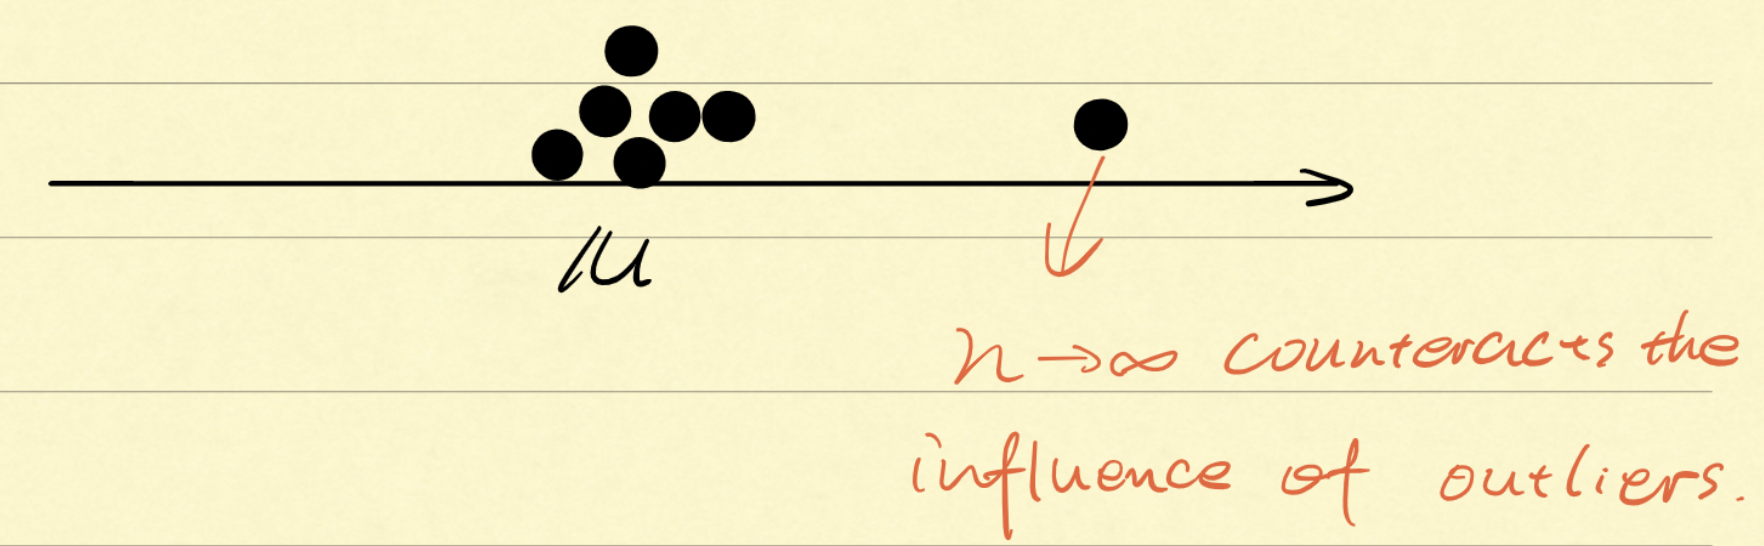
\includegraphics[scale=0.3]{wLLN.png}
        \caption{convergence in probability}
        \label{}
    \end{figure}\end{center}
    \item Strong Law of Large Numbers (sLLN)
    $$P(|\bar{x}-\mu|\geq\varepsilon\text{ as }n \rightarrow+\infty)=0,\ \forall \varepsilon>0$$
    \begin{center}\begin{figure}[htbp]
        \centering
        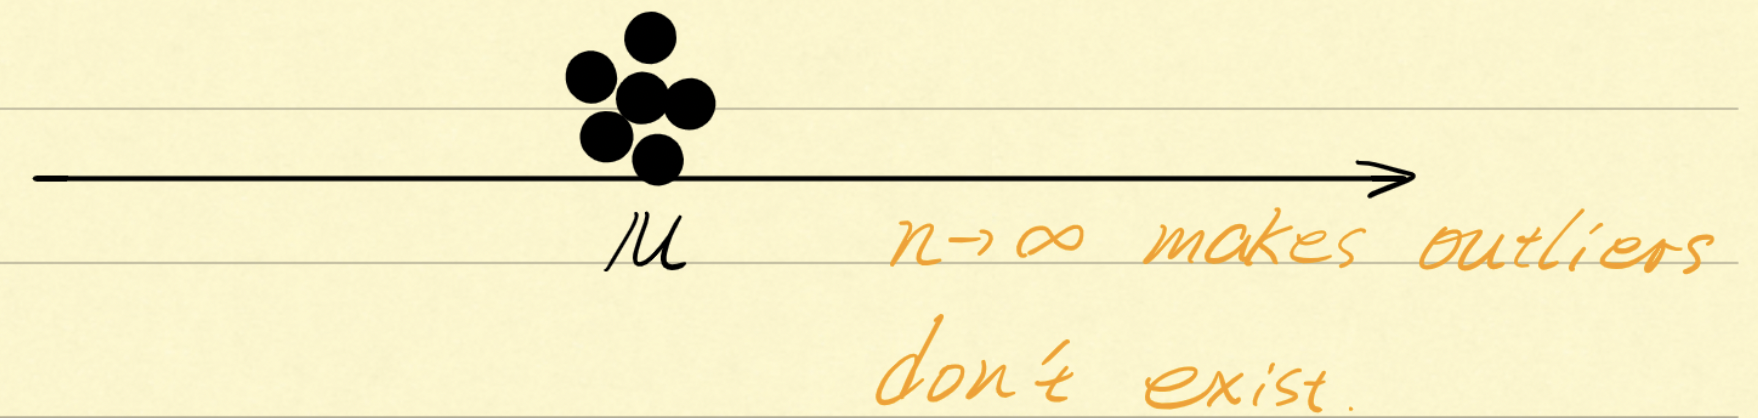
\includegraphics[scale=0.3]{sLLN.png}
        \caption{wp1(a.s.)}
        \label{}
    \end{figure}\end{center}
\end{enumerate}

\section{Central Limit Theorem (CLT)}
\begin{theorem}[Central Limit Theorem (CLT)]
    $$Z=\frac{\overline{X}-\mu}{\frac{\sigma}{\sqrt{n}}} \xrightarrow {D} N(0,1) \text{ when}\ n\to \infty$$
    $Z$ \underline{converges in distribution} to $N(0,1)$ as $n\to \infty$

    (converges in distribution: $P(\frac{\overline{X}-\mu}{\frac{\sigma}{\sqrt{n}}}\leq a)\rightarrow \frac{1}{\sqrt{2\pi}}\int_{-\infty}^ae^{-\frac{x^2}{2}}dx$)
\end{theorem}
\begin{proof}
    Prove the situation of $\mu=0,\sigma^2=1$, we can use linear transformations to get other situations.

    Moment-generating function(MGF) of $X_i$: $M_0(t)=E(e^{tX_i})$. $$M_0(0)=1,M_0'(0)=EX_i=0,M_0''(0)=EX_i^2=1$$
    Moment-generating function(MGF) of $\sqrt{n}\overline{X}$:
    \begin{equation}
        \begin{aligned}
            M_1(t)&=Ee^{t\sqrt{n}\overline{X}}=Ee^{t\frac{\sum_{i=1}^nX_i}{\sqrt{n}}}\\
            &=Ee^{t\frac{X_1}{\sqrt{n}}}\cdot Ee^{t\frac{X_2}{\sqrt{n}}}\cdots Ee^{t\frac{X_n}{\sqrt{n}}}\\
            &=[M_0(\frac{t}{\sqrt{n}})]^n
        \end{aligned}
        \nonumber
    \end{equation}
    \begin{equation}
        \begin{aligned}
            \lim_{n \rightarrow	\infty}\log M_1(t)&=\lim_{n \rightarrow	\infty}n\log M_0(\frac{t}{\sqrt{n}})\\
            &(\text{let }y=\frac{1}{\sqrt{n}})\\
            &=\lim_{y=0}\frac{\log M_0(yt)}{y^2}\\
            &(\text{L'Hôpital's rule})\\
            &=\lim_{y=0}\frac{t M'_0(yt)}{2y M_0(yt)}\\
            &(\text{L'Hôpital's rule})\\
            &=\lim_{y=0}\frac{t^2 M''_0(yt)}{2 M_0(yt)+2ytM'(yt)}\\
            &=\frac{t^2}{2}
        \end{aligned}
        \nonumber
    \end{equation}
    As we know the Moment-generating function(MGF) of $Z\sim N(0,1)$ is $M_Z(t)=\frac{t^2}{2}$.

    Hence, $M_1(t)=M_Z(t)$ i.e. $\frac{\overline{X}-\mu}{\frac{\sigma}{\sqrt{n}}} \xrightarrow {D} N(0,1)$ as $n \rightarrow\infty$
\end{proof}

\chapter{Metric Spaces Foundations \small{(Lec 01 @ ECON 240A)}}
\section{Probability Space}
\begin{definition}[Probability Space]
    \normalfont
    A \textbf{probability space} is triple $(S,\mathbb{B},P)$, where $S$ is a \underline{sample space}, $\mathbb{B}$ is a \underline{$\sigma-$algebra} of \underline{events}, and $P$ is a \underline{probability function}.
\end{definition}

\subsection{Sample Space}
\begin{definition}[Sample Space]
    \normalfont
    The \textbf{sample space} $S$ of an experiment is the list of all possible outcomes of the experiment. Elements $s\in S$ are called \underline{elementary outcomes}.
\end{definition}
\begin{example}
    \textbf{Coin Tossing:} $S=\{H,T\}$.
\end{example}

\subsection{$\sigma-$Algebra}
\begin{definition}[$\sigma-$Algebra of Events]
    \normalfont
    A subset (of $S$) $B\subseteq S$ is called an \textbf{event}.\\
    A \underline{collection $\mathbb{B}$ of events} is a \textbf{$\sigma-$algebra} \underline{if and only if}
    \begin{enumerate}
        \item $\emptyset\in \mathbb{B}$;
        \item $B\in \mathbb{B} \Rightarrow B^C \in \mathbb{B}$;
        \item $B_1,B_2,...\in \mathbb{B} \Rightarrow \cup_{i=1}^\infty B_i\in \mathbb{B}$.
    \end{enumerate}
\end{definition}
\begin{note}
    $S=\emptyset^C\in \mathbb{B}$.
\end{note}
\begin{example}
    \textbf{Coin Tossing:} $S=\{H,T\}$ has $\sigma-$algebra $\mathbb{B}=2^S=\{\emptyset,\{H\},\{T\},\{H,T\}\}$ (which is called the "discrete $\sigma-$algebra").
\end{example}

Standard $\sigma-$algebra when $S=\mathbb{R}$:
\begin{definition}[Borel $\sigma-$algebra]
    \normalfont
    The \textbf{Borel} $\sigma-$algebra on $\mathbb{R}$, $\mathcal{B}(\mathbb{R})$, is the smallest $\sigma-$algebra contains all open sets.
\end{definition}

\subsection{Probability Function}
\begin{definition}[Probability Function]
    \normalfont
    A function $P: \mathbb{B} \rightarrow [0,1]$ is a \textbf{probability function} \underline{if and only if}
    \begin{enumerate}
        \item $P(S)=1$;
        \item If $B_1,B_2,...\in \mathbb{B}$ are disjoint event, then $P(\cup_{i=1}^\infty B_i)=\sum_{i=1}^\infty P(B_i)$.
    \end{enumerate}
\end{definition}
\begin{note}
    \begin{enumerate}
        \item $\mathbb{B}$ is the domain of $P$.
        \item $S=\emptyset^C\in \mathbb{B}$ because $\mathbb{B}$ is a $\sigma-$algebra.
        \item $P(\emptyset)=0$ because $\emptyset$ and $S$ are disjoint, $P(\emptyset)+P(S)=P(\emptyset\cup S)=P(S)$.
    \end{enumerate}
\end{note}
\begin{example}
    \textbf{Coin Tossing:} $S=\{H,T\}$ has $\sigma-$algebra $\mathbb{B}=2^S=\{\emptyset,\{H\},\{T\},\{H,T\}\}$ (which is called the "discrete $\sigma-$algebra").
    \begin{equation}
        \begin{aligned}
            P(\emptyset)=0,P(\{H\})=P(\{T\})=\frac{1}{2},P(\{H,T\})=1
        \end{aligned}
        \nonumber
    \end{equation}
\end{example}

\begin{note}
    \textbf{Specifying $B\& P()$ in general:}
    \begin{enumerate}
        \item We don't specify $\mathbb{B}$ unless we have to.
        \item It suffices to specify $P()$ on a subset of $\mathbb{B}$. (In the example, we can only specify $P(\{H\})$ and $P(\{T\})$).
    \end{enumerate}
\end{note}
\begin{note}
    \textbf{Generalization:}\\
    If $S$ is \underline{(at most) countable}, then $\mathbb{B}=2^S$ is a standard choice. It suffices to specify $P(\{s\}), s\in S$.
\end{note}


\section{Random Variables}
\begin{definition}[Random Variable]
    \normalfont
    Let $(S,\mathbb{B},P)$ be a probability space. A \textbf{random variable} is a function $X: S \rightarrow \mathbb{R}$, which is "Borel measurable".
\end{definition}

\begin{note}
    Any random variable $X$ induces a probability space $(S_X,\mathbb{B}_X,P_X)$, where $S_X=\mathbb{R}$, $\mathbb{B}_X=\mathcal{B}(\mathbb{R})$, and $P_X=P\circ X^{-1}$ (that is, for all $B\in \mathcal{B}(\mathbb{R})$, $P_X(B)=P\circ X^{-1}(B)\triangleq P(\{s\in S: X(s)\in B\})$)
\end{note}

\begin{note}
    \textbf{Convention:} We work with $(S_X,B_X,P_X)$ and focus on specifying $P_X$.
\end{note}

\subsection{Represeting / Specifying $P_X$: Cumulative Distribution Function}
\begin{definition}[Cumulative Distribution Function]
    \normalfont
    The \textbf{cumulative distribution function} (cdf) of $X$ is the function $F_X: \mathbb{R} \rightarrow [0,1]$ given by $$F_X(x)=P_X((-\infty,x])=P(\{s\in S: X(s)\leq x\}), \forall x\in \mathbb{R}$$
\end{definition}

\begin{theorem}[Conditions of being a CDF]
    A function $F_X: \mathbb{R} \rightarrow [0,1]$ is cdf \underline{if and only if}
    \begin{enumerate}[(i).]
        \item $\lim_{x \rightarrow -\infty} F_X(x)=0$ and $\lim_{x \rightarrow \infty} F_X(x)=1$;
        \item $F_X$ is non-decreasing;
        \item $F_X$ is right-continuous.
    \end{enumerate}
\end{theorem}



\subsection{Correspondence Theorem; CDF $\Leftrightarrow$ Probability Function}
\begin{theorem}[Correspondence Theorem]
    Let $X\& Y$ be random variables and let the associated probability functions and cdfs be $P_X\& P_Y$ and $F_X\&F_Y$. Then, $$F_X=F_Y \textnormal{ \underline{if and only if} }P_X=P_Y$$
\end{theorem}
So, we can specify $P_X$ (on $\mathcal{B}(\mathbb{R})$) by specifying $F_X$ (on $\mathbb{R}$).

\begin{example}[Uniform Distribution]
    A random variable $X$ has a (standard) \underline{uniform} distribution, $X\sim U[0,1]$, if and only if
\end{example}



\chapter{Markov Chain}
\section{Definition}
For discrete state space $S$, a Markov Chain is a stochastic process $X_0,X_1,X_2,...$ such that
$$P(X_{n+1}=i|X_n=j,X_{n-1}=x_{n-1},...,X_0=x_0)=P(X_{n+1}=i|X_n=j)$$
for all $n\in \mathbb{Z}$ and $x_0,x_1,...,x_{n-1},i,j\in S$.

A MC is called \underline{time homogeneous} if $P(X_{n+1}=i|X_n=j)=P(X_1|X_0=j),\forall n\in \mathbb{Z}^+$ and $i,j\in S$ (we only consider time homogeneous MC).

The \textbf{transition probabilities} for a \underline{time homogeneous MC} can be written down as a matrix $P$ satisfying $P_{ij} = P (X_1 = j|X_0 = i)$. This matrix $P$ satisfies two properties:
\begin{enumerate}[(1)]
    \item $P_{ij}\geq 0$ for all $i,j\in S$.
    \item $\sum_{j\in S}P_{ij}=1$ for all $i\in S$.
\end{enumerate}
Any matrix satisfies the two properties is called a \textbf{stochastic matrix}.

\section{Matrix Computations}
Given a time homogeneous MC with initial distribution $X_0\sim\alpha\in [0,1]^{|S|}$ and transition matrix $P$.
\begin{lemma}[Distribution of Entire Sequence]
$$P(X_0=x_0,X_1=x_1,...,X_n=x_n)=P(X_0=x_0)P_{x_0,x_1}P_{x_1,x_2}...P_{x_{n-1},x_n}$$
\end{lemma}

\begin{lemma}[Markov Property]
    $$P(X_{t_n}=x_{t_n} | X_{t_{n-1}}=x_{t_{n-1}},...,X_{t_0}=x_{t_0})=P(X_{t_n}=x_{t_n}|X_{t_{n-1}}=x_{t_{n-1}})$$
\end{lemma}

\begin{lemma}[Transition Probability after $n$ states]
$$P(X_n=j|X_0=i)=(P^n)_{ij}$$
\end{lemma}
\begin{proof}
    $P(X_2=j|X_0=i)=\sum_{k\in S}P(X_2=j|X_1=k)P(X_1=k|X_0=i)=\sum_{k\in S}P_{kj}P_{ik}=(P^2)_{ij}$. Then prove by mathematical induction,
    $P(X_n=j|X_0=i)=\sum_{k\in S}P(X_n=j|X_{n-1}=k)P(X_{n-1}=k|X_0=i)=\cdots =(P^n)_{ij}$
\end{proof}

\subsection{Chapman Kolmogorov Equations (C-K Equations) $P(X_{n+m}=j|X_0=i)=(P^{m+n})_{ij}=\sum_{k\in S}(P^{m})_{ik}(P^{n})_{kj}$}
$m-$step transition probabilities from state $k$ to state $j$:
\begin{equation}
    P(X_{n+m}=j|X_0=i)=(P^{m+n})_{ij}=\sum_{k\in S}(P^{m})_{ik}(P^{n})_{kj}
\end{equation}
\begin{proof}
    $P(X_n=j|X_0=i)=\sum_{k\in S}P(X_{n+m}=j|X_{m}=k)P(X_{m}=k|X_0=i)=\sum_{k\in S}P(X_n=j|X_{0}=k)P(X_{m}=k|X_0=i)$
\end{proof}

\subsection{Marginal Distribution $P(X_n=j)=(\alpha P^n)_{j}$}
\begin{lemma}[Marginal Distribution]
    Given initial distribution $X_0\sim\alpha$ and transition matrix $P$. $\alpha$ is distribution vector ($1\times|S|$) with $\sum_{i\in S}{\alpha_i}=1$.
    $$P(X_n=j)=(\alpha P^n)_{j}$$
\end{lemma}
\begin{corollary}[Distribution of Subsequence]
    $$P(X_{t_{n}}=x_{t_{n}},X_{t_{n-1}}=x_{t_{n-1}},...,X_{t_0}=x_{t_0})=(\alpha P^{t_0})_{x_{t_0}}P^{t_1-t_0}_{x_{t_0},x_{t_1}}P^{t_2-t_1}_{x_{t_1},x_{t_2}}\cdots P^{t_{n}-t_{n-1}}_{x_{t_{n-1}},x_{t_{n}}}$$
\end{corollary}

\section{States, Class}
\subsection{Irreducible, Reducible}
\begin{enumerate}[$\bullet$]
    \item \underline{Accessible}: $j$ is accessible from $i$ if $\exists n$ s.t. $P_{ij}^n>0$.
    \item \underline{Communicate/Communication}: $i$ communicates $j$ ($i \leftrightarrow j$) if $j$ is accessible from $i$ and $i$ is accessible from $j$. (Reflexivity: $i \leftrightarrow i$; Symmetry: $i \leftrightarrow j$ $\Rightarrow$ $j \leftrightarrow i$; Transitivity: $i \leftrightarrow j$ and $j \leftrightarrow k$ $\Rightarrow$ $i \leftrightarrow k$.)
    \item \underline{(Communication) Class}: if $i \leftrightarrow j$, then states $i,j$ are said to be in the same \underline{(communication) class}. (Since communication is an equivalence relation, the state space can be partitioned into equivalence classes, called \textit{communication classes}.)
    \item \underline{Irreducible}: A Markov Chain that has \underline{only one class} is said to be \underline{irreducible}.
\end{enumerate}

\subsection{Recurrent, Transient}
\begin{enumerate}[$\bullet$]
    \item \underline{Recurrent State}: State $i$ is recurrent if $f_i=P($ever re-enter state $i$ if started in state $i)=1$. (the expected number of times it visits state $i$ is $\sum_{n=0}^\infty P_{ii}^n=+\infty$). (A MC is irreducible if all states are recurrent)
    \item \underline{Transient State}: State $i$ is transient if $f_i=P($ever re-enter state $i$ if started in state $i)<1$. (the expected number of times it visits state $i$ is $\sum_{n=0}^\infty P_{ii}^n<+\infty$; $P($visits state $i$ exactly $n$ times$)=f_i^{n-1}(1-f_i)$; The expected number is $\sum_{n=0}^\infty f_i^n(1-f_i)n={n=0}^\infty P_{ii}^n<\infty$).
    \item \underline{Transient Class}: A communicating class is called transient if starting from that class, with probability $1$ the MC leaves that class and never returns. The states of such a class are called transient states.
    \item \underline{Recurrent Class}: communicating class that is not transient.
    \begin{lemma}
        If $i$ is recurrent, $i\leftrightarrow j \Rightarrow$ $j$ is recurrent.
    \end{lemma}
    \begin{theorem}
        The states of a communication class are \underline{either all recurrent or all transient}.
    \end{theorem}
    \begin{corollary}
        For a \underline{finite irreducible} Markov chain, all states are recurrent.
    \end{corollary}
\end{enumerate}

\subsection*{Canonical Decomposition}
\begin{definition}
    A set of states $C$ is said to be \underline{closed} if no state outside of $C$ is accessible from any state in $C$. If $C$ is closed, then $$P_{ij} = 0,\ \forall i\in C,j\notin C$$
\end{definition}

\begin{lemma}
    (1) A communication class is \underline{closed} if it consists of all recurrent states.
    (2) A finite communication class is closed only if it consist of all recurrent states.
\end{lemma}
\begin{proof}
(1): if not closed, $\exists i\in C,j\notin C, P_{ij}>0$. $i$ shouldn't be accessible from $j$ since $i,j$ are not in one class. There exists positive probability that starting from $i$ then hit $j$ and never hit $i$ again, which contradicts to $i$ is recurrent. (2):According to former corollary, a finite class's all states are recurrent.
\end{proof}

\section{Periodicity}
Suppose $P$ is the transition matrix for an irreducible MC. For a given state $i$, we define the set $$J_i=\{n\geq 1:P^n(i,i)>0\}$$
$J_i$ is the set of times when it is possible for the MC to come back to $i$ starting from $i$ at time $0$. We define the \textbf{period} of a state $i$ is $$d(i)=gcd(J_i)$$
\subsection{Lemma: all states in an irreducible MC have the same period}
\begin{lemma}
    For an irreducible MC, all states have the same period.
\end{lemma}
\begin{proof}
    Let $d$ be a common divisor of $J_i$. Consider any other state $j$. We want to show $d$ is also the common divisor of $J_j$.
    
    Since the MC is irreducible, there exists $m$ and $n$ s.t. $P_{ij}^m>0$ and $P_{ji}^n>0$. Then $P_{ii}^{m+n}\geq P_{ij}^mP_{ji}^n >0 \Rightarrow m+n\in J_i$. $d$ should be a divisor of $m+n$.

    For any $l\in J_j$, $P_{ii}^{m+n+l}\geq P_{ij}^mP_{jj}^lP_{ji}^n >0 \Rightarrow m+n+l\in J_i$. $d$ divides $m+n+l$ $\Rightarrow$ $d$ divides $l$. Since $l$ can be any number in $J_j$, $d$ is a common divisor of $J_j$.
\end{proof}

\subsection{Periodic, Aperiodic}
A \underline{state} is \textbf{aperiodic} if period equals $1$, \textbf{periodic} otherwise.\\
A \underline{chain} is \textbf{aperiodic} if \underline{all} its states are aperiodic, \textbf{periodic} otherwise.

\section{Regular Matrix}
\subsection{Regular matrix: $\exists n\geq 1$ s.t. $P^n>0$}
A matrix $M$ is said to be positive if all the entries of $M$ are positive. We write $M > 0$.
\begin{definition}[Regular Transition Matrix]
    A transition matrix $P$ is said to be \underline{regular} if some power of $P$ is positive. That is, $P^n >0$, for some $n\geq 1$.
\end{definition}

\subsection{Lemma: Finite MC is Irreducible, Aperiodic $\Leftrightarrow$ has Regular transition matrix}
\begin{lemma}
    A finite MC is \textbf{irreducible} and \textbf{aperiodic} is equivalent to the transition matrix $P$ is \textbf{regular}.
\end{lemma}

We also call an MC is \textbf{ergodic} if it is \textbf{irreducible} and \textbf{aperiodic}.

\section{Eigenvalues of a Stochastic Matrix: $\lambda=1$ must exist and other $|\lambda|\leq 1$ (not equal when if regular matrix)}
\begin{lemma}
        A stochastic matrix $\boldsymbol{P}$ has an eigenvalue $\lambda^*=1$. All other eigenvalues $\lambda$ of $\boldsymbol{P}$ are such that $|\lambda| \leq 1$.
    
        If $\boldsymbol{P}$ is a regular matrix, then the inequality is strict. That is, $|\lambda|<1$ for all $\lambda \neq \lambda^*$.
\end{lemma}

\section{Long Run Behavior of Finite Markov Chains}
As $n \rightarrow \infty$, $P^n$:
\begin{enumerate}[(1)]
    \item Convergence. ($P^{n+1}=P^n$)
    \item Forgetting the initial states. (each row is identical)
\end{enumerate}


\subsection{Limiting Distribution}
\begin{definition}
    A MC is said to have a \textbf{limiting distribution} $\lambda$ if we have $$\lim_{n \rightarrow \infty}P_{ij}^n=\lambda_j,\ \forall i,j\in S$$
    An \underline{equivalent definition} is that for all initial distributions $X_0\sim \alpha$ and all $j\in S$ we have
    $$\lim_{n \rightarrow \infty}(\alpha P^n)_j=\lambda_j$$
\end{definition}

\textbf{Example: }$P=\begin{bmatrix}
    1-p&p\\
    q&1-q
\end{bmatrix}$. If $p+q=1$, each rows of $P$ is the same and $P^n=P$.

Assume $p+q\neq 1$,
\begin{equation}
    \begin{aligned}
        P^n_{11}&=P^{n-1}_{11}(1-p)+P^{n-1}_{12}q\\&=P^{n-1}_{11}(1-p)+(1-P^{n-1}_{11})q\\
        P^n_{11}&=\frac{q}{p+q}+\frac{p}{p+q}(1-p-q)^n \rightarrow \frac{q}{p+q}\text{ as }n \rightarrow \infty\\
        \lim_{n \rightarrow \infty}P^n&=\frac{1}{p+q}\begin{bmatrix}
            q&p\\
            q&p
        \end{bmatrix}
    \end{aligned}
    \nonumber
\end{equation}

\begin{lemma}
    If $\lambda$ is the limiting distribution for a MC with transition matrix $P$ then $\lambda$ satisfies the equation $$\lambda P=\lambda$$
\end{lemma}
\begin{proof}
    $(\lambda P)_j=\sum_{i\in S}\lambda_i P_{ij}=\sum_{i\in S}\lim_{n \rightarrow \infty}P_{ki}^nP_{ij}=\lim_{n \rightarrow \infty}\sum_{i\in S}P_{ki}^nP_{ij}=\lim_{n \rightarrow \infty}P_{kj}^{n+1}=\lambda_j$
\end{proof}

\subsection{Stationary Distribution}
\begin{definition}
    A distribution $\pi$ which satisfies the equation $$\pi P=\pi$$ is called a \textbf{stationary distribution} for the MC.
\end{definition}
\textbf{Note: }A limiting distribution $\lambda$ for the MC has to also be a stationary distribution. The converse is not always true.



\subsection{Limiting Distribution = Expected Proportion of time in each state}
The entries of the limiting distribution can also be interpreted as \textbf{the limit of the expected proportion of time the MC spends in each of the corresponding states.} For any state $j$, define the indicator random variable $I_k=1(X_k=j)$. Now define $$F_{n,j}=\frac{1}{n}\sum_{k=0}^{n-1}I_k$$
The random variable $F_{n,j}$ represents the proportion of time till time $n-1$ the MC spends in state $j$.

\begin{lemma}
    If $\lambda$ is the limiting distribution for a MC with transition matrix $P$ then $\lambda$ satisfies the equation $\lim_{n \rightarrow \infty}\mathbb{E}(F_{n,j}|X_0=i)=\lambda_j$ for all $j,i\in S$
\end{lemma}
\begin{proof}
    We can write $$\mathbb{E}(F_{n,j}|X_0=i)=\mathbb{E}\frac{1}{n}\sum_{k=0}^{n-1}\mathbb{E}(I_k|X_0=i)=\frac{1}{n}\sum_{k=0}^{n-1}P(X_k=j|X_0=i)=\frac{1}{n}\sum_{k=0}^{n-1}P_{ij}^k$$
    Therefore, taking limits we can conclude that $$\lim_{n \rightarrow \infty}\mathbb{E}(F_{n,j}|X_0=i)=\lim_{n \rightarrow \infty}\frac{1}{n}\sum_{k=0}^{n-1}P_{ij}^k=\lim_{n \rightarrow \infty}P_{ij}^n=\lambda_j$$
\end{proof}

\subsection{Fundamental Theorem for \underline{Irreducible, Aperiodic, Finite MC} (Regular transition matrix) $\Rightarrow $ $\exists$ unique limiting distribution $\pi$ and $\pi_j>0,\forall j$}
\begin{theorem}
    If $P$ is the transition matrix for an irreducible, aperiodic (finite) Markov chain then there exists a unique stationary distribution or a unique solution to the equation $\pi=\pi P$ which satisfies the following two properties:
    \begin{enumerate}[(1)]
        \item $\pi$ is the \textbf{limiting distribution} of the MC. ($\lim_{n \rightarrow \infty}\alpha P^n=\pi,\forall \alpha$ initial distribution)
        \item $\pi$ gives \textbf{positive} probability to each of the states. ($\pi_j>0,\forall j\in S$)
    \end{enumerate}
\end{theorem}


\subsection{Long run behavior for reducible and/or periodic chains}
\textbf{Question: What is the long run behavior for reducible and/or periodic chains?}\\
Assume $P$ is reducible with \underline{recurrent classes} $R_1, \ldots, R_r$ and \underline{transient classes} $T_1, \ldots, T_s$. Each recurrent class acts as a separate $\mathrm{MC}$ with transition matrix $P_1, \ldots, P_r$. Assume each $P_k$ is aperiodic. Then by the fundamental theorem, there exists $r$ different limiting distributions $\pi^1, \ldots, \pi^r$. The distribution $\pi^k$ is supported on its own recurrent class; i.e. $\pi^k(j)=0$ if $j \notin R_k .$ There are three cases to consider:
\begin{enumerate}
    \item If $i,j\in R_k$ (in the same recurrent class) then $$\lim_{n \rightarrow \infty}P_{ij}^n=\pi^k(j)$$
    \item \textbf{If $i$ is any transient state then eventually it ends up in one of the recurrent states.} Therefore, if $i,j$ are transient states then, $$\lim_{n \rightarrow \infty}P_{ij}^n=0$$
    \item Let $\alpha_k(i)$ for $k = 1,...,r$ be the probability that the chain starting in $i$ eventually ends up in a recurrent class $R_k$. (We will see later how to calculate $\alpha_k(i)$.) Once the chain reaches the recurrent class $R_k$, it will settle down to the limiting distribution on $R_k$. Therefore, we have for a transient state $i$ and $j \in R_k$, $$\lim_{n \rightarrow \infty}P_{ij}^n=\alpha_k(i)\pi^k(j)$$
\end{enumerate}
So, in this case there is a limit of $P^n$, but the limit will have different rows.

When an MC is irreducible but \textbf{periodic} (period $d>1$), we can show there is no \textbf{limiting distribution}. $P^n$ will keep switching according to whether $n|d$ has remainder $0,1,...,d-1$. Therefore, there cannot be a limit of $P^n$.

Although $\lim_{n \rightarrow \infty}P_{ij}^n$ doesn't exist in irreducible and periodic MC, $\lim_{n \rightarrow \infty}\frac{1}{n}\sum_{m=0}^{n-1}P_{ij}^m$ exists. It is the limit of the expected long run proportions of time spent in each state.

\subsection{Fundamental Theorem for \underline{Irreducible, Finite MC}: expected first return time $\mathbb{E}(T_j|X_0 = j)=\frac{1}{\pi_j}$}

$$T_j=\min\{n>0 : X_n = j\}$$ is the first time the chain returns to state $i$ after time $0$. This time is often also called the first passage time to the state $i$.

In a finite irreducible MC, $P(T_j<\infty)=1,\forall i$.
\begin{theorem}
    Assume that $X_0, X_1,...$ is a \underline{finite irreducible} Markov chain. For each state $j$, let $\mu_j = \mathbb{E}(T_j|X_0 = j)$ be the expected return time to $j$. Then, $\mu_j$ is finite, and there exists a unique \textbf{positive} stationary distribution $\pi$ such that $$\pi_j=\frac{1}{\mu_j},\forall j$$
    Furthermore, for all initial states $i$, limiting distribution on $j$ equals to the expected proportion of time spends in $j$: $$\pi_j=\lim_{n \rightarrow \infty}\frac{1}{n}\sum_{m=0}^{n-1}P_{ij}^m=\frac{1}{\mu_j},\forall j$$
\end{theorem}

\begin{proof}
    The sum of $k$ i.i.d. random variables $T_1+T_2+\cdots+T_k$ each of which follows the same distribution as $T$ conditional on $X_0=i$. For $k \rightarrow \infty$, by the Law of Large Numbers, $\lim_{k \rightarrow \infty}\frac{T_1+T_2+\cdots+T_k}{k} = \mathbb{E}(T|X_0=i)$.

    Consider this total time is $T_1+T_2+\cdots+T_k$ and the time we spent at $i$ is $k$, the expected proportion of time the chain spends in state $i$ is approximately $\lim_{k \rightarrow \infty}\frac{k}{T_1+T_2+\cdots+T_k}\approx \frac{1}{\mathbb{E}(T|X_0=i)}$. As we showed before, the expected proportion of time is $\pi_i$ $\Rightarrow \pi_i=\frac{1}{\mathbb{E}(T|X_0=i)}=\frac{1}{\mu_i},\forall i$
\end{proof}

\begin{example}[Two State MC]
    Consider the transition matrix $$P=\begin{bmatrix}
        1-p&p\\
        q&1-q
    \end{bmatrix}$$
\end{example}
Here, by the theorem $$\mu_0=\mathbb{E}[T_0|X_0=0]=\frac{1}{\pi(0)}=\frac{p+q}{q}$$

\section{Return Times and Absorption Probabilities}
\subsection{Expected Number of Visits to a Transient State: $E(Y_i|X_0 = j) = M_{ji} = (I-Q)^{-1}_{ji}$}
Let $P$ be the transition matrix of a $MC$. Suppose $P$ has some transient states and let $Q$ be the submatrix of $P$ which contains the rows and columns for the transient states. Hence, after reordering the states we can write $$P=\begin{bmatrix}
    \tilde{P}&0\\
    S&Q
\end{bmatrix}$$
Let $i$ be a transient state and let us define \textbf{a random variable which counts the total number of visits to the state $i$}$$Y_i=\sum_{n=0}^\infty \mathbf{1}_{X_n=i}$$
Since $i$ is transient, $Y_i<\infty$ w.p.1.
\begin{lemma}
    Let $Q$ denote the part of transition matrix indexed by the transient states. Define $M = (I-Q)^{-1}$. We have the following equality for any two transient states $i,j\in S$,
    $$E(Y_i|X_0 = j) = M_{ji}$$ Thus, the matrix $(I-Q)^{-1}$ gives the expected number of visits to a transient state $i$ when the $MC$ starts at a transient state $j$.
\end{lemma}
\begin{proof}
    We can write $$\mathbb{E}(Y_i|X_0 = j)=\sum_{n=0}^\infty P(X_n=i|X_0=j)=\sum_{n=0}^\infty P^n_{ji}=\sum_{n=0}^\infty Q^n_{ji}=M_{ji}$$
    The last equality holds because $I+Q+Q^2+\cdots=\frac{I(I-Q^\infty)}{1-Q}=(I-Q)^{-1}$
\end{proof}

We can also extend the equation: $$\mathbb{E}(Y_i|X_0 = j)=\mathbf{1}_{i=j}+\sum_{k\text{ transient}}\mathbb{E}(Y_i|X_1=k)Q_{jk}$$

\subsection{Expected Time till Absorption to a Recurrent Class: $\mathbb{E}(T_{abs}|X_0=j)=\sum_{i\in T_1\cup T_2\cup\cdots\cup T_s} M_{ji}$}
Let's define $$T_{abs}=\{\min_{n\geq 0}: X_n\in \text{a recurrent class}\}$$
which is \textbf{the waiting time till the chain enters a recurrent class}.
$T_{abs}$ also equals to the total time spent on transient states. $$T_{abs}=\sum_{i\in T_1\cup T_2\cup\cdots\cup T_s}Y_i$$
\begin{corollary}
    For any transient state $j\in S$, $$\mathbb{E}(T_{abs}|X_0=j)=\sum_{i\in T_1\cup T_2\cup\cdots\cup T_s} M_{ji}$$
\end{corollary}
\begin{example}
    Simple Random Walk (SRW) with absorbing boundaries on $\{0,1,2,3,4\}$
    $$P=\left(\begin{array}{ccccc}
    1 & 0 & 0 & 0 & 0 \\
    1 / 2 & 0 & 1 / 2 & 0 & 0 \\
    0 & 1 / 2 & 0 & 1 / 2 & 0 \\
    0 & 0 & 1 / 2 & 0 & 1 / 2 \\
    0 & 0 & 0 & 0 & 1
    \end{array}\right)$$
\end{example}
We can reorder it by $\{0,4,1,2,3\}$
$$P=\left(\begin{array}{ccccc}
    1 & 0 & 0 & 0 & 0 \\
    0 & 1 & 0 & 0 & 0 \\
    1 / 2 & 0 & 0 & 1 / 2 & 0 \\
    0 & 0 & 1 / 2 & 0 & 1 / 2 \\
    0 & 1 / 2 & 0& 1 / 2 & 0
    \end{array}\right)=\begin{bmatrix}
        I_{2\times 2}&	0\\
        S	& Q
    \end{bmatrix}$$
where $Q=\begin{bmatrix}
    0 & 1 / 2 & 0 \\
    1 / 2 & 0 & 1 / 2 \\
    0& 1 / 2 & 0
\end{bmatrix}$, then $$M=(I-Q)^{-1}=\begin{bmatrix}
    3/2 & 1 & 1/2 \\
    1 & 2 & 1 \\
    1/2& 1 & 3/2
\end{bmatrix}$$
Therefore $\mathbb{E}(Y_3|X_0=1)=\frac{1}{2}$, $\mathbb{E}(T_{abs}|X_0=1)=M_{11}+M_{12}+M_{13}=\frac{3}{2}+1+\frac{1}{2}=3$.

\subsection{Expected first return time (different initial state) = Time till Absorption}
We have computed $\mathbb{E}[T_i|X_0=i]=\frac{1}{\pi_i}$, we want to compute $$\mathbb{E}[T_i|X_0=j],i\neq j$$
\begin{enumerate}[\textbf{{Method}} 1:]
    \item Condition on first step: Let $a_j=\mathbb{E}[T_i|X_0=j]$
    \begin{equation}
        \begin{aligned}
            \mathbb{E}[T_i|X_0=j]&=P_{ji}\cdot 1+\sum_{k\neq i}P_{jk}\cdot(1+\mathbb{E}[T_i|X_0=k])\\
            &=1+\sum_{k\neq i}P_{jk}\cdot\mathbb{E}[T_i|X_0=k]\\
            \Rightarrow a_j&=1+\sum_{k\neq i}P_{jk}\cdot a_k
        \end{aligned}
        \nonumber
    \end{equation}
    Then the problem can be solved by solving the linear system for all $j\in S$.
    \item This problem can be transformed into computing the \textbf{expected time till absorption to $i$}. (we can let $i$ be an absorbing state)

    Reorder the transition matrix $P$ with $i$ being the first state and make $i$ an absorbing state $$P=\begin{bmatrix}
        P_{ii}& R\\
        S & Q
    \end{bmatrix} \Rightarrow \tilde{P}=\begin{bmatrix}
        1&0\\
        S&Q
    \end{bmatrix}$$
    Then $$\mathbb{E}[T_i|X_0=j]=\mathbb{E}[T_{abs}|X_0=j]$$
\end{enumerate}

\begin{example}
    Simple Random Walk (SRW) with reflecting boundaries on $\{0,1,2,3,4\}$
    $$P=\left(\begin{array}{ccccc}
    0 & 1 & 0 & 0 & 0 \\
    1 / 2 & 0 & 1 / 2 & 0 & 0 \\
    0 & 1 / 2 & 0 & 1 / 2 & 0 \\
    0 & 0 & 1 / 2 & 0 & 1 / 2 \\
    0 & 0 & 0 & 1 & 0
    \end{array}\right)$$
\end{example}
To compute $\mathbb{E}[T_0|X_0=j]$, we make $0$ an absorbing state:
$$P=\left(\begin{array}{ccccc}
    1 & 0 & 0 & 0 & 0 \\
    1 / 2 & 0 & 1 / 2 & 0 & 0 \\
    0 & 1 / 2 & 0 & 1 / 2 & 0 \\
    0 & 0 & 1 / 2 & 0 & 1 / 2 \\
    0 & 0 & 0 & 1 & 0
    \end{array}\right)=\begin{bmatrix}
        1&	0\\
        S&	Q
    \end{bmatrix}$$
where $Q=\left(\begin{array}{ccccc}
    0 & 1 / 2 & 0 & 0 \\
    1 / 2 & 0 & 1 / 2 & 0 \\
    0 & 1 / 2 & 0 & 1 / 2 \\
    0 & 0 & 1 & 0
    \end{array}\right)$, then we can calculate $$M=(I-Q)^{-1}=\left(\begin{array}{ccccc}
        2 & 2 & 2 & 1 \\
        2 & 4 & 4 & 2 \\
        2 & 4 & 6 & 3 \\
        2 & 4 & 6 & 4
        \end{array}\right)$$
Now we can compute $$\mathbb{E}[T_0|X_0=4]=M_{41}+M_{42}+M_{43}+M_{44}=16$$

\subsection{Probability of Eventually Entering a Given Recurrent Class: $A=(I-Q)^{-1}S=MS$}
In some MC, there are more than one recurrent class. e.g. $\{0\}.\{N\}$ in absorbing boundary exmaple. We want to know \textbf{what is the probability that the MC eventually ends up in a given recurrent class starting from a transient state $j$.}

We can create a modified $MC$ where each of the recurrent classes are seen as single states. Let these states be $r_1,...,r_k$ with $P (r_i, r_i) = 1,\forall i\in\{1,...,k\}$.

We denote all transient states as $t_1,...,t_s$. And the transistion matrix is expressed by $$P=\begin{bmatrix}
    I&0\\
    S&Q
\end{bmatrix}$$

Let $\alpha_{t_i,r_j}$ be the probability that the $MC$ strating at $t_i$ ends up at $r_j$. We set $\alpha_{r_i,r_i}=1$ and $\alpha_{r_i,r_j}=0,i\neq j$. Then, for any $t_i$, we can write by conditioning on the first step
\begin{equation}
    \begin{aligned}
        \alpha_{t_i,r_j}&=P(X_n=r_j\text{ eventually }|X_0=t_i)\\
        &=\sum_{x\in S}P(X_1=x|X_0=t_i)P(X_n=r_j\text{ eventually }|X_1=x)\\
        &=\sum_{x\in S}P(t_i,x)\alpha_{x,r_j}
    \end{aligned}
    \nonumber
\end{equation}
(this $S$ is the set of states.)
Let $A_{s\times k}$ be the matrix with $\alpha_{t_i,r_j}$ being entries. The above equation can be written as $$A=\left[S\ Q\right]\begin{bmatrix}
    I\\
    A
\end{bmatrix}=S+QA$$
$$\Rightarrow A=(I-Q)^{-1}S=MS$$
(this $S$ is the submartix in $P$)

\section{Examples of Finite MC}
\subsection{Gambler's Ruin}
\begin{example}[Gambler's Ruin]
    Consider the asymmetric Gambler's Ruin with winning probability $p\in (0,1)$. The state space is $\{0,1,...,N\}$.
\end{example}
Let $\alpha_j$ be the probability that the MC get absorbed in state $N$ stratinhg from state $j$. Clearly, $\alpha(0)=0,\alpha(N)=1$. For any $0<j<N$, we can condition on the first step to get
\begin{equation}
    \begin{aligned}
        \alpha(j)&=(1-p)\alpha(j-1)+p\alpha(j+1)\\
        \Rightarrow \alpha(j+1)-\alpha(j)&=\frac{1-p}{p}(\alpha(j)-\alpha(j-1))\\
        \Rightarrow 1=\alpha(N)-\alpha(0)&=\sum_{j=0}^{N-1}(\alpha(j+1)-\alpha(j))\\
        &=\sum_{k=0}^{N-1}\left(\frac{1-p}{p}\right)^k(\alpha(1)-\alpha(0))\\
        &=\left\{\begin{matrix}
            N\alpha(1),&p=0.5\\
            \frac{1-\left(\frac{1-p}{p}\right)^{N}}{1-\left(\frac{1-p}{p}\right)}\alpha(1),&p\neq 0.5
        \end{matrix}\right.
    \end{aligned}
    \nonumber
\end{equation}
$\alpha(1)=\alpha(1)-\alpha(0)=\left\{\begin{matrix}
    \frac{1}{N},&p=0.5\\
    \frac{1-\left(\frac{1-p}{p}\right)}{1-\left(\frac{1-p}{p}\right)^N},&p\neq 0.5
\end{matrix}\right.$. Then,
\begin{equation}
    \begin{aligned}
        \alpha(j)=\sum_{k=0}^{j-1}\left(\frac{1-p}{p}\right)^k(\alpha(1)-\alpha(0))=\left\{\begin{matrix}
            \frac{j}{N},&p=0.5\\
            \frac{1-\left(\frac{1-p}{p}\right)^{j}}{1-\left(\frac{1-p}{p}\right)^N},&p\neq 0.5
        \end{matrix}\right.
    \end{aligned}
    \nonumber
\end{equation}

\subsection{Simple Random Walk (SRW) on Undirected Graph}
Consider an undirected graph $(V,E)$. The state space is $V$. Let the degree $deg(i)$ of a vertex $i$ be the number of edges starting from $i$. Formally, we can write $deg(i) = \{j \in V : (i, j) \in E\}$. The transition matrix $P_{|V|\times|V|}$ is as follows. $$P_{ij}=\frac{1}{deg(i)}\mathbf{1}_{(i,j)\in E}$$

The MC is irreducible iff the graph is connected. When assuming connected we can compute the unique stationary distribution $$\pi(v)=\frac{deg(v)}{2|E|}=\frac{deg(v)}{\sum_{v\in V}deg(v)}$$
The period of the chain is either 1 or 2. The period is 2 if and only if the graph is bipartite, meaning that the set of vertices can be divided into two subsets and each edge in the graph goes from one subset to another.
\begin{center}\begin{figure}[htbp]
    \centering
    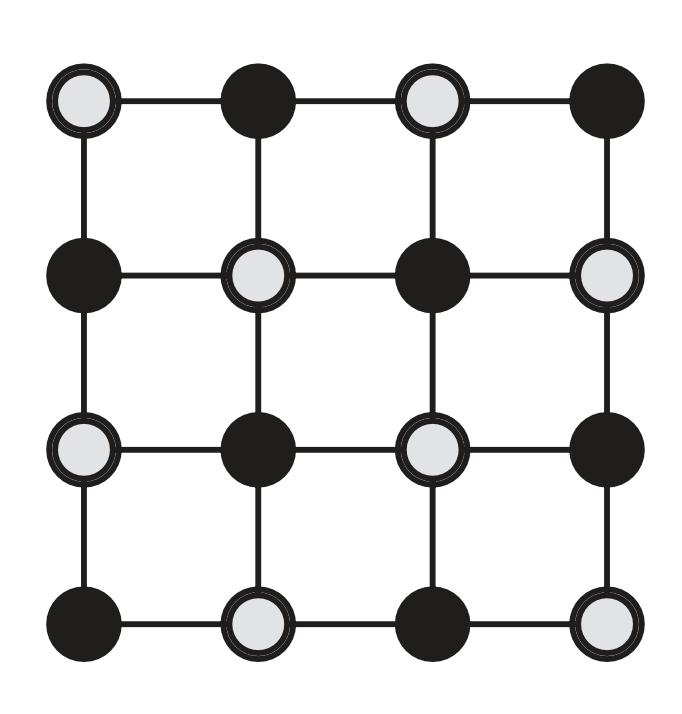
\includegraphics[scale=0.15]{bipartite.png}
    \caption{bipartite}
    \label{}
\end{figure}\end{center}
If the period is $1$ then $\pi$ is the limiting distribution for this chain. If the period is $2$ then $\pi$ can still be interpreted as the limiting expected fraction of time spent in each of the states.


\chapter{ Countably infinite MC}
Countably infinite MC: Markov Chain in countable infinite state space (e.g. $\mathbb{Z}$). The transition matrix $P$ is infinite large, but the sum of each row converges to $1$.
\subsection*{ Chapman Kolmogorov Equations (C-K Equations) also holds: $P(X_{n+m}=j|X_0=i)=(P^{m+n})_{ij}=\sum_{k\in S}(P^{m})_{ik}(P^{n})_{kj}$}
\textbf{Example}:
\begin{enumerate}[(1)]
    \item RW with partially reflecting boundary $S=\{0,1,2,...\}$, $P_{x,x-1}=1-p,P_{x,x+1}=p, P_{0,1}=p, P_{0,0}=1-p$.
    \item Queuing Model: $X_n=$ \# people at time $n$. $S=\{0,1,2,...\}$. $P(x,x-1)=q(1-p)$; $P(x,x+1)=(1-q)p$; $P(x,x)=pq+(1-p)(1-q)$; $P(0,0)=1-p$; $P(0,1)=p$.
\end{enumerate}

\subsection*{Difference: For the infinite, irreducible, and aperiodic MC, there may not exist stationary distribution.}
\begin{example}
    For Simple Random Walk: assume there exists a stationary distribution $\pi$, we have
    \begin{equation}
        \begin{aligned}
            \pi_j=\frac{1}{2}(\pi_{j-1}+\pi_{j+1}) \Rightarrow \pi_j-\pi_{j-1}=\pi_{j+1}-\pi_j
        \end{aligned}
        \nonumber
    \end{equation}
    Let the difference between $\pi_j-\pi_{j-1}=\varepsilon$, there doesn't exist solution to
    $$\sum_{i=0}^\infty \pi_i=1; \pi_i=i \varepsilon, i=0,1,...$$
\end{example}

\section{Recurrence and Transience}

\subsection{Recurrent or Transient State}
Suppose the first return time $T_j=\min\{n>0:X_n=j\}$.

Let the probability of the chain return to $j$ given $X_0=j$ is $$f_j=P(T_j<\infty|X_0=j)$$

\begin{definition}
    A state $j$ is \textbf{recurrent} if $f_j=1$ and \textbf{transient} if $f_j<1$.
\end{definition}

\subsection{Recurrent or Transient Class}
(Also class properties: states of a class should be all recurrent or all transient)
\begin{lemma}
    If $i,j$ are in the same class, $i$ is recurrent $\Leftrightarrow$ $j$ is recurrent.
\end{lemma}
\begin{proof}
    Suppose $i$ is recurrent, $P(T_i<\infty|X_0=i)=1$. Since $i\sim j$, $\exists k>0,P_{ij}^k>0$.

    Suppose $P(T_j<\infty|X_0=j)<1$ i.e., $P(T_j=\infty|X_0=j)>0$. Then,
    \begin{equation}
        \begin{aligned}
            P(T_i=\infty|X_0=i)&\geq P(T_i=\infty|X_0=j)P_{ij}^k\\
            &=P(T_i=\infty| T_j=\infty, X_0=j)P(T_j=\infty| X_0=j)P_{ij}^k>0
        \end{aligned}
        \nonumber
    \end{equation}
\end{proof}

\subsection{Lemma: Transient Class $\Leftrightarrow$ $\sum_{n=0}^\infty P_{i,i}^n<\infty$}
\begin{lemma}
    An irreducible MC is \textbf{transient} \underline{if and only if} the expected number of visits to a state is finite; i.e. $$\sum_{n=0}^\infty P_{i,i}^n<\infty$$
\end{lemma}
\begin{proof}
    Let the total number of visits $i$ in infinite time is $Y_i=\sum_{n=0}^\infty \mathbf{1}_{X_n=i}$. The expected number is $\mathbb{E}[Y_i|X_0=i]=\sum_{n=0}^\infty P_{i,i}^n$.
    
    $\Leftarrow$: If $i$ is recurrent, the expected total number to visits $i$ in infinite time should be infinite.
    Then, the MC can be proved to be transient if $\mathbb{E}[Y_i|X_0=i]=\sum_{n=0}^\infty P_{i,i}^n<\infty$.

    $\Rightarrow$: Suppose $i$ is transient, let $f_i=P(T_i=\infty|X_0=i)=q>0$ (Probability of not return). Then, the expected number of \underline{returns} to $i$ is (follows geometric distribution)
    \begin{equation}
        \begin{aligned}
            \sum_{n=0}^\infty (1-q)^nqn=q(1-q)\frac{\partial \left(-\sum_{n=0}^\infty(1-q)^n\right)}{\partial q}=q(1-q)\frac{\partial \left(-\frac{1}{q}\right)}{\partial q}=\frac{1-q}{q}
        \end{aligned}
        \nonumber
    \end{equation}
    which also equals to $\mathbb{E}[Y_i|X_0=i]-1 \Rightarrow \mathbb{E}[Y_i|X_0=i]=\frac{1}{q}<\infty$
\end{proof}

\subsection{Recurrence/Transience of Simple Random Walk on Lattice}
\textbf{Is the $d$ dimensional SRW recurrent or transient?}

We can first consider $d=1$ case. We want to compute the probability of returning to state $0$ (the same as others). For $2n$ steps trajectories, there are $\begin{pmatrix}
    2n\\
    n
\end{pmatrix}$ trajectories that can return to $0$ and each has probability $\frac{1}{2^{2n}}$.
$$P_{0,0}^{2n}=\begin{pmatrix}
    2n\\
    n
\end{pmatrix}\frac{1}{2^{2n}}=\frac{(2n)!}{n!n!2^{2n}}$$
\textbf{Using Stirling's formula:} $n!\sim\sqrt{2\pi n}\left(\frac{n}{e}\right)^n$ that is $\lim_{n \rightarrow \infty}\frac{n!}{\sqrt{2\pi n}\left(\frac{n}{e}\right)^n}=1$
$$P_{0,0}^{2n}\sim\frac{2\sqrt{\pi n}\left(\frac{2n}{e}\right)^{2n}}{2\pi n\left(\frac{n}{e}\right)^{2n}2^{2n}}=\frac{1}{\sqrt{\pi n}}$$
So the $\sum_{n=N}^\infty P_{0,0}^{2n}=\sum_{n=N}^\infty\frac{1}{\sqrt{\pi}}n^{-\frac{1}{2}}=\infty$.

\textbf{Note:} $n^{-\alpha}$ diverges when $\alpha\in (0,1]$ and converges when $\alpha>1$.

For $d$ dimensions, $$P_{0,0}^{2n}\sim n^{-\frac{d}{2}}$$

\begin{lemma}
    SRW is recurrent when $d=1,2$; SRW is transient when $d\geq 3$.
\end{lemma}



\subsection{Null and Positive Recurrence}
$\mu_j= \mathbb{E}[T_j|X_0=j]$
\begin{definition}
    A state $j$ is \textbf{positive recurrent} if it is recurrent and $\mu_j<\infty$. A state $j$ is \textbf{null recurrent} if it is recurrent and $\mu_j=\infty$.
\end{definition}
\textbf{Example of null recurrent:} $P(T_i=n)=\frac{1}{n(n+1)}=\frac{1}{n}-\frac{1}{n+1},n\geq 1$.
\begin{equation}
    \begin{aligned}
        f_i&=\sum_{n=1}^\infty P(T_i=n)=\sum_{n=1}^\infty\left(\frac{1}{n}-\frac{1}{n+1}\right)\Rightarrow \text{ recurrent}\\
        \mu_i&=\sum_{n=1}^\infty nP(T_i=n)=\sum_{n=1}^\infty\frac{1}{n+1}=\infty\Rightarrow \text{ null recurrent}
    \end{aligned}
    \nonumber
\end{equation}

\subsection{Stationary Distribution and Limiting Distribution}
Limiting distribution $$\lim_{n \rightarrow \infty}P^{n}_{y,x}=\pi(x),\ \forall x,y\in S$$
Obviously, when a chain is transient, $\lim_{n \rightarrow \infty}P^{n}_{y,x}=0$, there will be no limiting distribution. We can also know $\lim_{n \rightarrow \infty}P^{n}_{y,x}=0$ when the chain is null recurrent.

\begin{lemma}
    For an irreducible MC, $\lim_{n \rightarrow \infty}P^{n}_{y,x}=0$ for each $x,y\in S$ \textbf{if and only if} the chain is transient or null recurrent.
\end{lemma}

\begin{theorem}[Fundamental Theorem for General Discrete Markov Chains]
    An \textbf{irreducible, positive recurrent} MC has a \textbf{unique stationary distribution} $\pi$ (which is positive everywhere) solving the equation
    $$\sum_{y\in S}\pi(y)P(y,x)=\pi(x),\ \forall x\in S$$
    $\pi(j)$ equals to the \textbf{expected visiting time} at $j$ $$\lim_{n \rightarrow \infty}\frac{1}{n}\sum_{k=0}^{n-1}P_{ij}^k=\pi(j)$$
    If in addition, the MC is \textbf{aperiodic}, then $$\lim_{n \rightarrow \infty}P_{ij}^n=\pi(j)$$
    The stationary distribution $\pi$ is also \textbf{inversely} related to the \textbf{expected first return times}. $$\pi(j)=\frac{1}{\mathbb{E}(T_j|X_0=j)}=\frac{1}{\mu_j}$$
    Furthermore, if the irreducible chain is not positive recurrent then there does not exist a stationary distribution.
\end{theorem}

\textbf{Note:} we can prove a MC is not positive recurrent by showing the MC doesn't have a stationary distribution.



\section{Differences between Finite and (Countably) Infinite Markov Chains}
\begin{enumerate}
    \item An irreducible MC with finite $S$ has to be recurrent. An irreducible MC with infinite $S$ could be recurrent or transient.
    \item An irreducible MC with finite $S$ has to be positive recurrent. An irreducible recurrent MC with infinite $S$ could be positive recurrent ($\mathbb{E}[T_j|X_0=j]<\infty$) or null recurrent ($\mathbb{E}[T_j|X_0=j]=\infty$).
    \item An irreducible MC with finite $S$ always has a unique stationary distribution. An irreducible recurrent MC with infinite $S$ has a (unique) stationary distribution if and only if the MC is positive recurrent.
\end{enumerate}

\chapter{Branching Process}
(Sir Francis Galton, 1873) It is a stochastic model for population growth. Let $X_n$ denote the number of individuals at time $n$. At each time interval, each individual will produce a random number of offsprings and then die.

\textit{Two Assumptions:}
\begin{enumerate}[(1)]
    \item Each individual produces offspring with the same probability distribution: there are given non-negative numbers $p_0, p_1, ...$ summing up to $1$ so that the probability of an individual producing $k$ children is $p_k$.
    \item The individuals reproduce independently.
\end{enumerate}

We want to know
\begin{center}
    \textit{"What is the probability that the population eventually becomes extinct?"}
\end{center}

The number of individuals at time $n$, $X_n$ is a MC with state space $S = \{0,1,2,...\} = \mathbb{Z}_+$. Note that $0$ is an absorbing state. Suppose $X_n = k$. Then k individuals produce offspring for the next generation. Let $Y_1,...,Y_k$ be i.i.d random variables with $P(Y_1 = j) = p_j$. Then we can write the transition probabilities as $$P_{k,j}=P(Y_1+\cdots+Y_k=j)$$
Since $P(X_1=0|X_0=i)=p_0^i>0$ for each $i>0$, the \underline{any state $i>0$ must be transient}. From this, it can be shown that, with probability $1$, the chain must either get absorbed in $0$ eventually or approach $\infty$.

\section{Extinction Probability in a Branching Process}
\subsection{Expectation $\mathbb{E}X_n=\mu^n \mathbb{E}X_0$}
The mean number of offsprings produced by an individual: $$\mu=\sum_{i=0}^\infty i p_i$$
The mean number of individuals in generation $n$,
\begin{equation}
    \begin{aligned}
        \mathbb{E}X_n=\sum_{k=0}^\infty P(X_{n-1}=k)\mathbb{E}(X_n|X_{n-1}=k)=\sum_{k=0}^\infty P(X_{n-1}=k)k\mu=\mu \mathbb{E}X_{n-1}
    \end{aligned}
    \nonumber
\end{equation}
Then, we can get $$\mathbb{E}X_n=\mu^n \mathbb{E}X_0$$

\subsection{Lemma: $\mu<1$ $\Rightarrow$ $P(extinction)=1$}
\begin{lemma}
    If $\mu < 1$, then probability of extinction is $1$.
\end{lemma}
\begin{proof}
    We know the event $\{X_{n-1}=0\}\subseteq \{X_{n}=0\}$
    $$P(extinction)=P(\cup_{n=0}^\infty\{X_n=0\})=\lim_{n \rightarrow \infty}P(X_n=0)$$
    \begin{equation}
        \begin{aligned}
            P(X_n\geq 1)=\sum_{k=1}^\infty P(X_n=k)\leq \sum_{k=1}^\infty kP(X_n=k)= \mathbb{E}X_n
        \end{aligned}
        \nonumber
    \end{equation}
    Now, the probability of survival
    \begin{equation}
        \begin{aligned}
            \lim_{n \rightarrow \infty}P(X_n\geq 1)&\leq \lim_{n \rightarrow \infty} \mathbb{E}X_n=\lim_{n \rightarrow \infty} \mu^n \mathbb{E}X_0=0\\
            \Rightarrow \lim_{n \rightarrow \infty}P(X_n\geq 1)&=0
        \end{aligned}
        \nonumber
    \end{equation}
    Then we can conclude $$P(extinction)=\lim_{n \rightarrow \infty}P(X_n=0)=1-\lim_{n \rightarrow \infty}P(X_n\geq 1)=1$$
\end{proof}

If $\mu = 1$, the expected population size remains constant while if $\mu > 1$, the expected population size grows.

\subsection{Variance: $Var X_n=n\sigma^2$ if $\mu=1$; $Var X_n=\sigma^2\mu^{n-1}\frac{\mu^n-1}{\mu-1}$ if $\mu\neq 1$}
Let's calculate the variance of $X_n$. We denote the variance of the number of offsprings produced by an individual by $\sigma^2$. By the law of total variance,
\begin{equation}
    \begin{aligned}
        Var X_n&=Var(\mathbb{E} X_n|X_{n-1})+\mathbb{E}Var(X_n|X_{n-1})\\&=Var(\mu X_{n-1})+ \mathbb{E}(\sigma^2 X_{n-1})\\&=\mu^2 Var(X_{n-1})+\sigma^2 \mu^{n-1}\mathbb{E}X_0
    \end{aligned}
    \nonumber
\end{equation}
(Assuming $X_0=1$ with probability $1$)
\begin{equation}
    \begin{aligned}
        Var X_n=\left\{\begin{matrix}
            n\sigma^2,&\mu=1\\
            \sigma^2\mu^{n-1}\frac{\mu^n-1}{\mu-1},&\mu\neq 1
        \end{matrix}\right.
    \end{aligned}
    \nonumber
\end{equation}



\subsection{Extinction probability $\rho=1$ if $\mu\leq 1$; $\rho<1$ if $\mu>1$}

To avoid trivial cases, we assume 1.$p_0>0$; 2. $p_0+p_1<1$.

Let $a_n(k)=P(X_n=0|X_0=k)$ and let $a(k)=\lim_{n \rightarrow \infty}a_n(k)$ denote the probability that the population dies out eventually assuming that $X_0=k$.

Since all $k$ individuals act independently, we must have $$a(k)=a(1)^k$$

We simply denote $a(1)$ by $\rho$.
\begin{equation}
    \begin{aligned}
        \rho=a(1)=P(extinction|X_0=1)=\lim_{n \rightarrow \infty}P(X_n=0|X_0=1)
    \end{aligned}
    \nonumber
\end{equation}
By conditioning on the first step, we can write
\begin{equation}
    \begin{aligned}
        \rho=\sum_{k=0}^\infty P(X_1=k|X_0=1)P(extinction|X_1=k)=\sum_{k=0}^\infty p_k\rho^k=\psi(\rho)
    \end{aligned}
    \nonumber
\end{equation}
where $\psi:[0,1] \rightarrow \mathbb{R}$ is given by $\psi(z)=\sum_{k=0}^\infty p_k z^k$. Then the $\rho$ satisfies $z=\psi(z)$

\begin{definition}
    If a random variable $X$ takes values in $\mathbb{Z}$, the \textbf{probability generating function (pgf)} of $X$ is the function $\psi : [0,1] \rightarrow \mathbb{R}$ given by $$\psi(s)=\psi_X(s)=\mathbb{E}(s^X)=\sum_{k=0}^\infty s^k P(X=k)$$
\end{definition}

We now note some important properties of the function $\psi$.
\begin{enumerate}
    \item $\psi'(x)=\sum_{k=1}^\infty x^{k-1}k p_k>0$ for $x\in (0,1)$ $\Rightarrow$ $\psi$ is an \textbf{increasing} function.
    \item $\psi^{''}(x)=\sum_{k=2}^\infty x^{k-2}k(k-1) p_k>0$ for $x\in (0,1)$ $\Rightarrow$ $\psi$ is a \textbf{convex} function.
    \item $\psi(0)=p_0>0$
    \item $\psi(1)=1$
    \item $\psi'(1)=\sum_{k=1}^\infty k p_k=\mu$
    \item \textbf{Probability Generating Functions characterize the distribution}: if two discrete random variables have their pgf the same then they have the same distribution.
    \item $\psi_{X+Y}(s)=\mathbb{E}(s^{X+Y})=\mathbb{E}(s^X)\mathbb{E}(s^Y)=\psi_X(s)\psi_Y(s)$
\end{enumerate}

\begin{center}\begin{figure}[htbp]
    \centering
    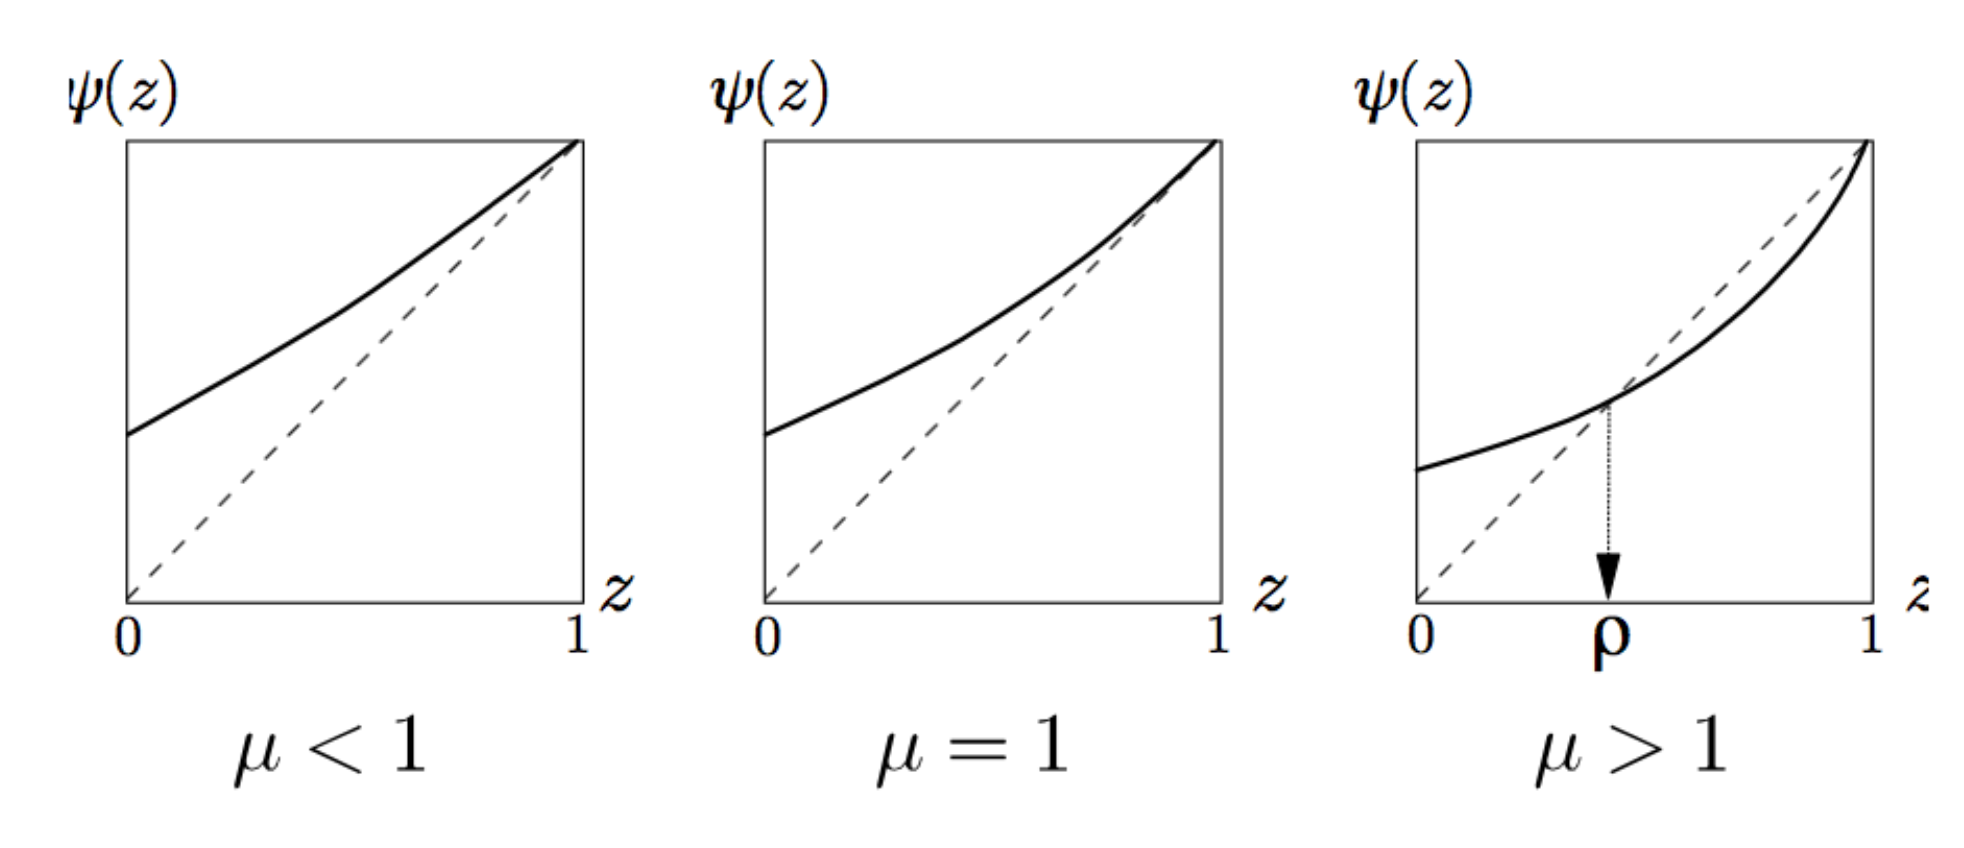
\includegraphics[scale=0.2]{pgf.png}
    \caption{Fixed Point of pgf}
    \label{}
\end{figure}\end{center}

From the pictures we can find that $\rho=1$ is the unique fixed point of $\psi(z)$ when $\mu\leq 1$ and there exists another fixed point $\rho=r\in (0,1)$ when $\mu>1$.

Suppose $\mu>1$. Denote $q_n=a_n(1)=P(X_n=0|X_0=1)$, where $\lim_{n \rightarrow \infty}q_n=\rho$. Defining $r$ to be the smaller solution of $\psi(z)=z$.

We want to prove $q_n\leq r$, $\forall n\geq 0$. Prove by induction:
\begin{enumerate}
    \item Let $q_0=0$.
    \item Assume that $q_n\leq r$,
    \begin{equation}
        \begin{aligned}
            q_{n+1}&=P(X_{n+1}=0|X_0=1)=\sum_{k=0}^\infty P(X_{n+1}=0|X_1=k)p_k\\&=\sum_{k=0}^\infty P(X_{n}=0|X_0=k)p_k=\sum_{k=0}^\infty q_n^k p_k=\psi(q_n)
        \end{aligned}
        \nonumber
    \end{equation}
    Since $\psi$ is increasing, we have $q_{n+1}=\psi(q_n)\leq \psi(r)=r$
\end{enumerate}

\begin{theorem}
    If $\mu<1$ or $\mu=1$, the extinction probability $\rho=1$. If $\mu>1$, then the extinction probability $\rho<1$ and equals to the unique root of $z=\psi(z),z\in (0,1)$.
\end{theorem}

\begin{example}
    $p_0=\frac{1}{8},p_1=\frac{3}{8},p_2=\frac{3}{8},p_3=\frac{1}{8}$.
\end{example}
Since $\mu=\frac{3}{2}>1$, we can solve $\frac{1}{8}+\frac{3}{8}r+\frac{3}{8}r^2+\frac{1}{8}r^3=r$. Because $r=1$ is always a solution $\Rightarrow (r-1)(r^2+4r-1)=0$ $r^*=\sqrt{5}-2$.

\subsection{$G_n(s)=G_{n-1}(\psi(s))=\psi(\psi(\psi(\cdots\psi(s)\cdots)))=\psi(G_{n-1}(s))$}
For $n\geq 0$, let
\begin{equation}
    \begin{aligned}
        G_n(s)=\sum_{k=0}^\infty s^k P(Z_n=k)
    \end{aligned}
    \nonumber
\end{equation}
be the generating function of the $n^{th}$ generation size $Z_n$. $$G_1(s)=\psi(s)$$

We have
\begin{equation}
    \begin{aligned}
        G_n(s)&=\psi_{Z_n}(s)=\mathbb{E}(s^{Z_n})= \mathbb{E}\left(\mathbb{E}(s^{\sum_{k=1}^{z}X_k})|Z_{n-1}=z\right)\\
        &=\mathbb{E}\left(\prod_{k=1}^{z}\mathbb{E}(s^{X_k})|Z_{n-1}=z\right)=\mathbb{E}\left((\psi(s))^{z}|Z_{n-1}=z\right)\\
        &=\mathbb{E}\left[(\psi(s))^{Z_{n-1}}\right]=G_{n-1}(\psi(s))
    \end{aligned}
    \nonumber
\end{equation}

Since $G_2(s)=G_1(\psi(s))=\psi(\psi(s))=\psi(G_1(s))$, we can infer
\begin{equation}
    \begin{aligned}
        G_n(s)=G_{n-1}(\psi(s))=\psi(\psi(\psi(\cdots\psi(s)\cdots)))=\psi(G_{n-1}(s))
    \end{aligned}
    \nonumber
\end{equation}




















\chapter{Time Reversible Markov Chains}
\section{Definition: Local Balance $\pi(i)P(i,j)=\pi(j)P(j,i),\forall i,j\in S$}
\begin{definition}
    We say that a $M C$ is \textbf{time reversible} if, for each $n \geq 1$, the distribution of $\left(X_0, \ldots, X_n\right)$ is the same as the distribution of $\left(X_n, \ldots, X_0\right)$. Equivalently, for any $x_0, \ldots, x_n \in \mathcal{S}$ we have
    $$
    P\left(X_0=x_0, X_1=x_1, \ldots, X_n=x_n\right)=P\left(X_n=x_0, X_{n-1}=x_{n-1}, \ldots, X_0=x_n\right) .
    $$
    In words, the probability of a given trajectory is the same as the probability of the reverse trajectory.
\end{definition}

\begin{lemma}[Local Balance]
    The Markov chain $X_0, X_1, . . .$ is time-reversible \textbf{if and only if} the distribution $\pi$ of $X_0$ satisfies the condition
    \begin{equation}
        \begin{aligned}
            \pi(i)P(i,j)=\pi(j)P(j,i),\forall i,j\in S
        \end{aligned}
        \nonumber
    \end{equation}
\end{lemma}

\section{Discussion about Local Balance}
\subsection{Flow: $Flow(A,B)=\sum_{i\in A}\sum_{j\in B}\pi(i)P_{ij}$}
\begin{definition}
    For a distribution $\pi$ on the state space $S$ and any two subsets of the state space $A, B$ define the \textbf{Flow}
    \begin{equation}
        \begin{aligned}
            Flow(A,B)=\sum_{i\in A}\sum_{j\in B}\pi(i)P_{ij}
        \end{aligned}
        \nonumber
    \end{equation}
\end{definition}

\subsection{Lemma: $Flow(A,A^c)=Flow(A^c,A)$ for any subset $A\subset S$}
\begin{lemma}
    $Flow(A,A^c)=Flow(A^c,A)$ for any subset $A\subset S$.
\end{lemma}
\begin{proof}
    \begin{equation}
        \begin{aligned}
            Flow(A,A^c)&=\sum_{i\in A}\sum_{j\in A^c}\pi(i)P_{ij}=\sum_{i\in A}\pi(i)(1-\sum_{j\in A}P_{ij})=\sum_{i\in A}\pi(i)-\sum_{i\in A}\sum_{j\in A}\pi(i)P_{ij}\\\
            Flow(A^c,A)&=\sum_{i\in A^c}\sum_{j\in A}\pi(i)P_{ij}=\sum_{j\in A}(\pi(j)-\sum_{i\in A}\pi(i)P_{ij})=\sum_{j\in A}\pi(j)-\sum_{j\in A}\sum_{i\in A}\pi(i)P_{ij}
        \end{aligned}
        \nonumber
    \end{equation}
\end{proof}

\subsection{Lemma: Local balance $\Rightarrow$ $\pi$ is stationary}
\begin{lemma}
    If the local balance equations "$\pi(i)P(i,j)=\pi(j)P(j,i),\forall i,j\in S$" hold then $\pi$ is stationary.
\end{lemma}
\begin{proof}
    $$(\pi P)_i=\sum_{j\in S}\pi_j P_{ji}=\sum_{j\in S}\pi_i P_{ij}=\pi_i$$
\end{proof}

\subsection{Lemma: All stationary birth and death chains are reversible}
\begin{lemma}
    All stationary birth and death chains are reversible. (i.e. For a MC with $P_{i,j}=0,\forall |i-j|>1$, $\pi(i)P(i,j)=\pi(j)P(j,i),\forall i,j\in \mathbb{Z}_+$)
\end{lemma}
\begin{proof}
    It is enough to show the equation holds when $j = i + 1$. For $A=\{0,1,2,...,i\}$,
    \begin{equation}
        \begin{aligned}
            &Flow(A,A^c)=\sum_{0\leq k\leq i}\sum_{j>i}\pi(k)P_{kj}=\pi(i)P_{i,i+1}\\
            =&Flow(A^c,A)=\sum_{j>i}\sum_{0\leq k\leq i}\pi(j)P_{jk}=\pi(i+1)P_{i+1,i}
        \end{aligned}
        \nonumber
    \end{equation}
\end{proof}

\section{Example: Random Walk on an Undirected Graph}
\begin{lemma}
    Any stationary random walk on a weighted undirected graph is time reversible. On the other hand, any time reversible MC can be thought of as a random walk on a weighted undirected graph.
\end{lemma}
\begin{proof}
    Consider a RW on a weighted undirected graph $G=(V, W)$. Recall that every potential edge or a pair of states $i, j$ has some weight $W_{i j} \geq 0$. Since the graph is undirected this means that the edge weights $W_{i j}=W_{j i}$ are symmetric. The transition probabilities are $P_{v,u}=\frac{W_{vu}}{\sum_{v\in S} W_{vu}}$, where $S=\{v: W_{uv}\neq 0\}$. By the symmetric property, $P_{v,u}=\frac{W_{vu}}{\sum_{v\in S} W_{vu}}=\frac{W_{uv}}{\sum_{v\in S} W_{uv}}$. Let's denote $W=\sum_{(i, j) \in V \times V} W_{i j}$.

    We know from an earlier lecture that the stationary distribution is given by $\pi(v)=$ $\frac{\sum_{v \in \mathcal{S}} W_{u v}}{W}$. Let's now check that this $\pi$ satisfies the local balance.
    $$
    \pi(v) P_{v, u}=\frac{\sum_{v \in \mathcal{S}} W_{u v}}{W} \frac{W_{u v}}{\sum_{v \in \mathcal{S}} W_{u v}}=\frac{W_{u v}}{W} .
    $$
    The right hand side above is symmetric in $u, v$ so local balance must hold.
    On the other hand, lets consider a time reversible MC. Build a graph where the set of vertices is same as the state space of this MC. Define the edge weights to be $W_{i j}=\pi_i P_{i j}$. Since local balance holds we have $W_{i j}=W_{j i}$. Now we can imagine a random walk on this weighted undirected graph. What is the transition probability $Q$ of this random walk? It has to be
    $$
    Q_{u v}=\frac{W_{u v}}{\sum_{v \in \mathcal{S}} W_{u v}}=\frac{\pi(v) P_{v, u}}{\sum_{u \in \mathcal{S}} \pi(v) P_{v, u}}=P_{v, u} .
    $$
    Therefore, this random walk describes the same $\mathrm{MC}$ as the original one.

\end{proof}





\chapter{Markov Chain Monte Carlo (MCMC)}
Given a probability distribution $\pi$, the goal of MCMC is to simulate a random variable $X$ whose distribution is $\pi$.

The MCMC algorithm constructs an ergodic (irreducible and aperiodic) Markov chain whose limiting distribution is the desired $\pi$.

\section{Strong Law of Large Numbers for Markov Chains}
\begin{theorem}
    Assume that $X_0,X_1,...$ is an ergodic Markov chain  with stationary distribution $\pi$. Let $r$ be a bounded and real-valued function. Let $Y$ be a random variable with distribution $\pi$. Then, with probability $1$,
    \begin{equation}
        \begin{aligned}
            \lim_{n \rightarrow \infty}\frac{r(X_1)+\cdots+r(X_n)}{n}=\mathbb{E}_Y[r(Y)]
        \end{aligned}
        \nonumber
    \end{equation}
    where $\mathbb{E}_Y[r(Y)]=\sum_{j}r(j)\pi_j$
\end{theorem}
What different to LLN is $X_1,..,X_n$ are not i.i.d.

\section{Example of Designing MC}
\begin{enumerate}
    \item All binary sequence consisted of $0$ or $1$ of length $d$, $S=\{0,1\}^d$, $|S|=2^d$. $\pi$ is a uniform distribution on all $S$, obviously, each sequence has probability $\frac{1}{2^d}$. We can use a MC of tossing a coin to simulate it.
    \item All binary sequence consisted of $0$ or $1$ of length $d$ and \textbf{no consecutive 1}, $B=\{0,1\}^d$. $\pi$ is a uniform distribution on all $B$, but it is hard to get the $|B|$ in this situation.
    \begin{enumerate}[-]
        \item \textbf{Ejection Sampling:} sample a random sequence from $S$, eject the sequence is not in $B$.
        (issue: usually the $|B|$ is small compared to $|S|$, the method works badly, e.g. when $d=100$, $|B|\sim 10^{21}, |S|\sim 10^{30}$)
        \item \textbf{MCMC:} Given sequence $(x_1,...,x_d)$, pick a coordinate at random (with probability $\frac{1}{d}$ each). If the coordinate is $1$ then flip it to $0$. If the coordinate is $0$, then flip it to $1$ if this results in a sequence in $B$, otherwise do not flip it.
        
        We can identify the facts of the MC:
        \begin{enumerate}[(1)]
            \item The MC is irreducible;
            \item Period = 1;
            \item For $i\neq j$, $P_{ij}=P_{ji}=1$ or $=0$ $\Rightarrow$ local balance is satisfied for $\pi$
        \end{enumerate}
        The above three facts imply that the uniform distribution $\pi$ is the stationary and limiting distribution of this chain
    \end{enumerate}
    Interested in calculating the expected number of $1$ in a sequence $\mathbb{E} f(\pi)$ (the function of counting $1$ in a sequence is represented by $f(\cdot)$), suppose $X\sim \text{Unif}(B)$. We can calculate $$\frac{f(X_1)+\cdots+f(X_n)}{n} \rightarrow \mathbb{E}f(\pi)$$
\end{enumerate}

\section{Metropolis Hastings Algorithm}
Given a proposal chain $T$, we want local balance holds: $$\pi_i T_{ij}=\pi_j T_{ji}$$
However, sometimes the equation may not hold. We modify the transition matrix by $$\pi_i T_{ij}A_{ij}=\pi_j T_{ji},\text{ where }A_{ij}=\frac{\pi_j T_{j i}}{\pi_i T_{i j}}$$
Assume at time $n$, the chain is at state $i$ or equivalently, $X_n=i$. The next step of the chain $X_{n+1}$ is determined by the following two-step procedure.
\begin{enumerate}
    \item Choose a new state according to the transition matrix $T$. That is, choose $j$ with probability $T_{i j}$. State $j$ is called the proposal state.
    \item Define
    $$
    A_{i j}=\min \left\{1, \frac{\pi_j T_{j i}}{\pi_i T_{i j}}\right\}\quad \text{(Actually, it is fine to let $A_{ij}=\frac{\pi_j T_{j i}}{\pi_i T_{i j}}$)}
    $$
    Generate a uniformly random number between 0 and 1 as $U \sim U(0,1)$. If $U \leq A_{i j}$ then $j$ is accepted as the next state of the chain. If $U>A_{i j}$ then $j$ is not accepted as the next state of the chain and $X_{n+1}=i$.
\end{enumerate}
\begin{lemma}
    Let $P$ denote the modified transition matrix of the Metropolis-Hastings algorithm. Then $\pi$ satisfies local balance with respect to $P$.
\end{lemma}

Therefore, $\pi$ is stationary and if the MC with the new transition dynamics is ergodic then $\pi$ is limiting. If we start out with an irreducible chain then the final chain is also irreducible.

\textbf{Note:} If the proposal chain is ergodic so is the resulting Metropolis Hastings chain.


\subsection{Example of generate standard normal distribution with uniform}
Suppose we want to generate a standard normal random variable using only a uniform random number generator. The target density function is $\pi(t)=\frac{\exp \left(-t^2 / 2\right)}{\sqrt{2 \pi}}$. For the proposal distribution, we choose the uniform distribution of length 2 centered at the current state. From state $s$, the proposal chain moves to $t$, where $t$ is uniformly distributed on $(s-1, s+1)$. The conditional density $T(s, t)=1 / 2$ if $|s-t| \leq 2$ and 0 otherwise. The acceptance function then becomes
$$
A(s, t)=\min \left\{1, \frac{\pi(t) T_{t s}}{\pi(s) T_{s t}}\right\}=\min \left\{1, \exp \left(\left[-t^2+s^2\right] / 2\right)\right\}
$$

\subsection{Without MCMC: Box Muller Transform}
There are methods to sample exactly from the standard normal distribution without using MCMC. For any continuous random variable $X$ with CDF $F$, the random variable $F^{-1}(U)$ has the same distribution as $X$ when $U \sim Unif(0,1)$. For the standard normal the function $F^{-1}$ is not available in closed form. There is another method called the \textit{Box Muller Transform}.

The basic idea is as follows. $X, Y$ are two independent standard normal random variables if and only if $(R, \Theta)$ are independent, $\Theta$ follows $Unif(0,2 \pi)$ and $R^2$ follows a Chi Squared distribution with degrees of freedom $2$ which is the same as the Exponential Distribution with mean $2$. Here $(R, \Theta)$ are the polar coordinates corresponding to the cartesian coordinates $(X, Y)$. Therefore, to sample two independent standard normals it is enough to sample $R$ and $\Theta$. Sampling $\Theta \sim \operatorname{Unif}(0,2 \pi)$ is easy and sampling $R=\sqrt{R^2} \sim \sqrt{\text { Exponential }(2)}$ is easy by the inverse CDF method.

\section{Gibbs Sampling}
\textit{Gibbs sampling} is a MCMC algorithm for obtaining approximate draws from a joint distribution, based on sampling from \textbf{conditional distributions} one at a time: at each stage, one variable is updated (keeping all the other variables fixed) by drawing from the conditional distribution of that variable given all the other variables. This approach is especially useful in problems where the conditional distributions are simple enough to simulate from but the overall joint distribution is complicated.

There are several forms of Gibbs samplers, depending on the order in which updates are done. We will introduce two major kinds of Gibbs sampler: systematic scan, in which the updates sweep through the components in a deterministic order, and random scan, in which a randomly chosen component is updated at each stage.

\subsection{ Systematic scan Gibbs sampler}
Let $X$ and $Y$ be discrete r.v.s with joint PMF $p(x,y) = P(X = x, Y = y)$. We wish to construct a two-dimensional Markov chain $(X_n,Y_n)$ whose stationary distribution is $p$.
The \textit{systematic scan Gibbs sampler} proceeds by updating the $X$ component and the $Y$ component in alternation. If the current state is $\left(X_n, Y_n\right)=\left(x_n, y_n\right)$, then we update the $X$ component while holding the $Y$ component fixed, and then update the $Y$ component while holding the $X$ component fixed:
\begin{enumerate}
    \item Draw a value $x_{n+1}$ from the conditional distribution of $X$ given $Y=y_n$, and set $X_{n+1}=x_{n+1}$
    \item Draw a value $y_{n+1}$ from the conditional distribution of $Y$ given $X=x_{n+1}$, and set $Y_{n+1}=y_{n+1}$
    \item Repeating steps 1 and 2 over and over, the stationary distribution of the chain $\left(X_0, Y_0\right)$, $\left(X_1, Y_1\right)$, $\left(X_2, Y_2\right)$, $\ldots$ is $p$.
\end{enumerate}

Why is the last statement true? Suppose we are updating the $X$ coordinate. Suppose $(X, Y) \sim p$. We transition to $\left(X^{\prime}, Y\right)$ where $X^{\prime}$ is drawn from the conditional distribution of $p$ given $Y$. So we can write
$$
P\left(X^{\prime}=x, Y=y\right)=P\left(X^{\prime}=x \mid Y=y\right) P(Y=y)=p(x \mid y) p(y)=p(x, y)
$$
The second equality is true because $(X, Y) \sim p$. The above display shows that $p$ is stationary for this chain.

\subsection{ Random Scan Gibbs sampler}
Similarly, we wish to construct a two-dimensional Markov chain $(X_n,Y_n)$ whose stationary distribution is $p$. However, each move of the \textit{random scan Gibbs sampler} picks a uniformly random component and updates it, according to the conditional distribution given the other component:
\begin{enumerate}
    \item Choose which component to update, with equal probabilities.
    \item If the $X$-component was chosen, draw a value $x_{n+1}$ from the conditional distribution of $X$ given $Y=y_n$, and set $X_{n+1}=x_{n+1}, Y_{n+1}=y_n$. Similarly, if the $Y$-component was chosen, draw a value $y_{n+1}$ from the conditional distribution of $Y$ given $X=x_n$, and set $X_{n+1}=x_n, Y_{n+1}=y_{n+1}$.
    \item Repeating steps 1 and 2 over and over, the stationary distribution of the chain $\left(X_0, Y_0\right)$, $\left(X_1, Y_1\right)$, $\left(X_2, Y_2\right)$, $\ldots$ is $p$.
\end{enumerate}
Gibbs sampling generalizes naturally to higher dimensions. If we want to sample from a $d$ dimensional joint distribution, the Markov chain we construct will be a sequence of $d$ dimensional random vectors. At each stage, we choose one component of the vector to update, and we draw from the conditional distribution of that component \textbf{given the most recent values of the other components}. We can either cycle through the components of the vector in a systematic order, or choose a random component to update each time.

The Gibbs sampler is less flexible than the Metropolis-Hastings algorithm in the sense that we don't get to choose a proposal distribution; this also makes it simpler in the sense that we don't have to choose a proposal distribution. The flavors of Gibbs and Metropolis-Hastings are rather different, in that Gibbs emphasizes conditional distributions while Metropolis-Hastings emphasizes acceptance probabilities. But the algorithms are closely connected, as we show below.

\begin{theorem}[Random scan Gibbs as Metropolis-Hastings]
    The random scan Gibbs sampler is a special case of the Metropolis-Hastings algorithm, in which the proposal is always accepted. In particular, it follows that the stationary distribution of the random scan Gibbs sampler is as desired.
\end{theorem}
The random scan Gibbs sampler proposal chain satisfies local balance.

\subsection{Example: Bivariate Normal Distribution}
Consider a bivariate standard normal distribution with a correlation of $\rho$. If $(X, Y)$ has a bivariate normal distribution then the conditional distribution of $X \mid Y=y$ is normal with mean $\rho y$ and variance $1-\rho^2$. Similarly, the conditional distribution of $Y \mid X=x$ is normal with mean $\rho x$ and variance $1-\rho^2$. Therefore, we can implement Gibbs sampler by simply generating normal random variables each time. We write the steps when using the deterministic scan version, although the random scan version is equally applicable.
\begin{enumerate}[(a)]
    \item Initialize $\left(x_0, y_0\right)=(0,0)$. Also initialize $n=1$.
    \item Generate $x_n \sim N\left(\rho y_{n-1}, 1-\rho^2\right)$.
    \item Generate $y_n \sim N\left(\rho x_n, 1-\rho^2\right)$.
    \item Update $n=n+1$.
    \item Return to Step $(b)$.
\end{enumerate}
\textbf{Remark.} Recall that there is a simple exact method to sample standard Bivariate Normal with correlation $\rho$. First sample two i.i.d $Z_1, Z_2 \sim N(0,1)$. Now let $X=Z_1$ and $Y=\rho Z_1+\sqrt{1-\rho^2} Z_2$.

\subsection{Example: Potts model (Ising model)}
The Potts model is a generalization of the Ising model, and is used regularly in statistical physics and computer science. Fix a graph $G=(V, E)$. Let $\sigma: V \rightarrow\{1, \cdots, q\}$ for some $q>1$. The Potts model is a probability distribution on such functions $\sigma$, and is specified as follows:
$$
\pi(\sigma)=\frac{1}{Z} \exp \left(\beta \sum_{i \sim j} \mathbf{1}\left(\sigma_i=\sigma_j\right)\right)
$$
where $\beta \in \mathbb{R}$ is a constant. Derive a Gibbs sampler for the Potts model.

Cycle over the coordinates. At each step, given $\sigma_{-i} := (\sigma_1,...,\sigma_{i-1},\sigma_{i+1},...,\sigma_n)$, sample $\sigma_i$ from the distribution
\begin{equation}
    \begin{aligned}
        \pi_i(k\mid\sigma_{-i})=\frac{1}{Z} \exp \left(\beta \sum_{j \sim i} \mathbf{1}\left(\sigma_j=k\right)\right)
    \end{aligned}
    \nonumber
\end{equation}
\begin{enumerate}[(a)]
    \item Initialize $\sigma_{0,j}=1,\forall j\in V$. Also initialize $n=1$.
    \item For $i$ in $V$: Generate $\sigma_{n,i} \sim \pi_i(k\mid\sigma_{n-1,-i})$.
    \item Update $n=n+1$.
    \item Return to Step $(b)$.
\end{enumerate}


\section{A Linear Algebraic Condition for Convergence}
Let's assume a finite reversible ergodic $M C$ with transition matrix $P$ and stationary distribution $\pi$. Suppose the cardinality of the state space is $k$. Let $Q$ be the diagonal matrix with diagonals square root of the entries of $\pi$. Let $A=Q P Q^{-1}$.
We can check that
$$
A_{i j}=\sum_{r=1}^k \sum_{s=1}^k Q_{i r} P_{r s} Q_{s j}^{-1}=Q_{i i} P_{i j} Q_{j j}^{-1}=\sqrt{\frac{\pi_i}{\pi_j}} P_{i j}
$$
Since the chain is reversible, we obtain
$$
A_{i j}=\sqrt{\frac{\pi_i}{\pi_j}} P_{i j}=\frac{\pi_i P_{i j}}{\sqrt{\pi_i \pi_j}}=\frac{\pi_j P_{j i}}{\sqrt{\pi_i \pi_j}}=A_{j i} .
$$
We will now use some Linear Algebra facts which we state below.
\begin{enumerate}[(1)]
    \item \textbf{Spectral decomposition theorem:} A real symmetric matrix $A$ can be orthogonally diagonalized, that is $$A=S D S^T$$ where $S$ is an orthonormal real matrix and $D$ is a diagonal real matrix with $A$'s eigenvalues as entries.
    \item Since $P=Q^{-1}AQ$, $P$ has the same eigenvalues as $A$.\\($det(P-\lambda I)=0 \Rightarrow 0=det(QP-\lambda Q)=det(AQ-\lambda Q)=0 \Rightarrow det(A-\lambda I)=0$)
    \item Since $P$ is ergodic (irreducible and aperiodic), $P$ has regular transition matrix. Then the eigenvalues can be written $$1=\lambda_1>\lambda_2\geq \lambda_3\geq \cdots\geq \lambda_k>-1$$
\end{enumerate}
Now we can write
$$
P=Q^{-1} A Q=Q^{-1}\left(S D S^T\right) Q=\left(Q^{-1} S\right) D\left(S^T Q\right)
$$
where $D$ has diagonal entries $1, \lambda_2, \ldots, \lambda_k$. Now, for any integer $n \geq 1$, we can compute $P^n=\left(Q^{-1} S\right) D^n\left(S^T Q\right)$. Taking the $i j$ th entry,
$$
P_{i j}^n=\sum_{t=1}^k\left(Q^{-1} S\right)_{i t} \lambda_t^n\left(S^T Q\right)_{t j}=\sqrt{\frac{\pi_j}{\pi_i}} \sum_{t=1}^k \lambda_t^n S_{i t} S_{j t}=\sqrt{\frac{\pi_j}{\pi_i}} S_{i 1} S_{j 1}+\sqrt{\frac{\pi_j}{\pi_i}} \sum_{t=2}^k \lambda_t^n S_{i t} S_{j t}
$$
Since $\lim _{n \rightarrow \infty} P_{i j}^n=\pi_j$ this means that $\sqrt{\frac{\pi_j}{\pi_i}} S_{i 1} S_{j 1}=\pi_j$ and moreover we can write
$$
\left|P_{i j}^n-\pi_j\right|=\left|\sqrt{\frac{\pi_j}{\pi_i}} \sum_{t=2}^k \lambda_t^n S_{i t} S_{j t}\right| \leq \underbrace{\sqrt{\frac{\pi_j}{\pi_i}} \sum_{t=2}^k\left|S_{i t} S_{j t}\right|}_{T_1} \underbrace{\max _{2 \leq t \leq n}\left|\lambda_t^n\right|}_{T_2} .
$$
The $T_1$ term is a constant and does not change with $n$. The term $T_2$ decreases geometrically because it is strictly less than $1$. The above display shows that the rate of convergence of a reversible ergodic $\mathrm{MC}$ is governed by how close the second largest (in absolute value) eigenvalue is to 1 in absolute value. This gap between 1 and the second-largest eigenvalue (in absolute value) is often called the spectral gap and if this gap is not too small then the convergence happens exponentially fast.

\textbf{Remark.} In principle, for any MCMC method we can just compute its spectral gap to know how fast it will converge. In practice, this is often not possible as the state space is too large to compute eigenvalues of the transition matrix.









\chapter{Poisson Process}

\section{Basics of Poisson Process}
\subsection{Counting Process}
\begin{definition}[discrete time]
    A counting process $(N_t)_{t\geq0}$ is a collection of non-negative integer valued random variables such that if $0 \leq s \leq t$, then $N_s \leq N_t$.
\end{definition}
We use $N(t)$ to denote counting process.

\subsection{Poisson Distribution}
\begin{lemma}
    If $\lambda_n$ is a sequence of positive numbers with $\lim_{n \rightarrow \infty}\lambda_n=\lambda$ then $$\lim_{n \rightarrow \infty}\left(1-\frac{\lambda_n}{n}\right)^n=e^{-\lambda}$$
\end{lemma}

\begin{theorem}
    If $n \rightarrow  \infty$ and $p \rightarrow 0$ in such a way that $Np \rightarrow \lambda$, then the Binomial distribution with parameters $(N,p)$ converges to the Poisson $\lambda$ distribution.
\end{theorem}
Consider a unit time (the unit is divided into $n$ equal subparts, $n \rightarrow \infty$), there is an event may occur with every subpart, the number of the event happens should follow binomial distribution $B(n,p)$, where $n \rightarrow \infty, p \rightarrow 0$; $\lambda=n\cdot p$ is the expected number of events in this period of time.

The probability the number of the event happens:
\begin{equation}
    \begin{aligned}
        \Pr(X=k)&=\lim_{n \rightarrow\infty} \binom{n}{k} (\frac{\lambda}{n})^k(1-\frac{\lambda}{n})^{n-k}\\
        &=\lim_{n \rightarrow\infty} \frac{n!}{(n-k)!k!} (\frac{\lambda}{n})^k(1-\frac{\lambda}{n})^{n}(1-\frac{\lambda}{n})^{-k}\\
        &=\lim_{n \rightarrow\infty}\frac{n!}{(n-k)!k!} (\frac{\lambda}{n})^k e^{-\lambda}\\
        &=\frac{\lambda^k e^{-\lambda}}{k!}\lim_{n \rightarrow\infty}\frac{n!}{(n-k)!n^k}\\
        &=\frac{\lambda^k e^{-\lambda}}{k!}\lim_{n \rightarrow\infty}
        \frac{n}{n}\frac{n-1}{n}\cdots \frac{n-k+1}{n}\\
        &=\frac{\lambda^k e^{-\lambda}}{k!}
    \end{aligned}
    \nonumber
\end{equation}
For a Poisson distribution $Pois(\lambda)$. $\lambda$ is frequency of the event, i.e., the average number of event happens within unit time.
$$\Pr(X{=}k)= \frac{\lambda^k e^{-\lambda}}{k!},\ k=0,1,2,3...$$
$$E(X)=Var(X)=\lambda$$


\subsection{Definition of Poisson Process}
\begin{definition}[Definition 1 of PP]
        A \textbf{Poisson Process with parameter $\lambda$} is a counting process $\left(N_t\right)_{t \geq 0}$ with the following properties:
        \begin{enumerate}
            \item $N_0=0$.
            \item For all $t>0, N_t$ has a Poisson distribution with parameter $\lambda t$. $N_t\sim Pois(\lambda t)$.
            $$P(N_t=k)=\frac{(\lambda t)^{k}e^{-\lambda t}}{k!}$$
            \item For all $s, t>0$, the increment $N_{t+s}-N_s$ has the same distribution as $N_t$. This property is called \textbf{stationary increments}.
            \item For $0 \leq q<r \leq s<t$, the increments $N_t-N_s$ and $N_r-N_q$ are independent random variables. This property is called \textbf{independent increments}.
        \end{enumerate}
\end{definition}
The stationary increments property says that the distribution of the number of arrivals in an interval only depends on the length of the interval. The independent increment property says that the number of arrivals on disjoint intervals are independent random variables. Since $N_t$ has a Poisson distribution, $\mathbb{E} N_t=\lambda t$. So, we expect about $\lambda t$ arrivals in $t$ time units. We say that the rate of arrivals is $\lambda$.
\begin{proposition}[Translated PP]
    Let $N_t$ be a PP with parameter $\lambda$. For $t_0 > 0$, let $$\tilde{N}_t=N_{t+t_0}-N_{t_0}$$ for $t\geq 0$. Then $(\tilde{N}_t)_{t\geq 0}$ is a Poisson process with parameter $\lambda$.
\end{proposition}

\section{Inter-Arrival Times}
\subsection{First arrival time: Exponential distribution $Exp(\lambda)$}
For a PP with parameter $\lambda$, let $X$ denote the time of the first arrival. Then, the event $\{X>t\}$ happens if and only if there are no arrivals in $[0, t]$. Thus, for any $t \geq 0$,
$$
P(X>t)=P\left(N_t=0\right)=e^{-\lambda t}
$$
Hence, $X$ has an exponential distribution with parameter $\lambda$ or mean $\frac{1}{\lambda}$.
$$f_{X}(t)=\lambda e^{-\lambda t},\ \textnormal{for } t>0$$
$$\mathbb{E}(X)=\frac{1}{\lambda};\ Var(X)=\frac{1}{\lambda^2}$$
Recall that the pdf of the Exponential distribution with parameter $1$ is given by $f(x)=\exp (-x)$ for $x>0$, and an Exponential with parameter $\lambda$ can always be represented as $\frac{1}{\lambda} \operatorname{Exp}(1)$.

\begin{definition}[Definition 2 of PP]
        Let $X_1, X_2, \ldots$ be a sequence of i.i.d exponential random variables with parameter $\lambda$ or mean $\frac{1}{\lambda}$. For $t>0$, let
        $$
        N_t=\max \left\{n: X_1+\cdots+X_n \leq t\right\}
        $$
        with $N_0=0$. Then $\left(N_t\right)_{t \geq 0}$ defines a Poisson process with parameter $\lambda$.
\end{definition}
\begin{claim}[ Simulation 1.]
    The above definition leads to a direct method for simulating a Poisson Process in $[0, t]$.
\end{claim}

\subsection{$k^{th}$ arrival time: Gamma distribution $Gamma(n,\lambda)$}

\textbf{Remark.} The above definition says that a PP is a counting process for which interarrival times are i.i.d exponential random variables. Let $S_n=X_1+\cdots+X_n$ for $n=1,2, \ldots$ We call $S_1, S_2, \ldots$ as arrival times of the process, where $S_k$ is the $k^{th}$ arrival. Furthermore, $X_k=S_k-S_{k-1}$ is the $k^{th}$ interarrival time between the $(k-1)^{th}$ arrival and the $k^{th}$ arrival, with $S_0=0$.

For a PP, each arrival time $S_n$ is a sum of $n$ i.i.d exponential inter arrival times. A sum of i.i.d exponential ($\lambda$) distribution has a $Gamma(n, \lambda)$ distribution. The pdf of a Gamma $(n, \lambda)$ is $$f(t;n,\lambda)=\frac{\lambda^n t^{n-1}e^{-\lambda t}}{(n-1)!},\ \textnormal{for } t>0$$
The cdf is,
\begin{equation}
    \begin{aligned}
        {\displaystyle F(t;n ,\lambda )=1-\sum _{i=0}^{n -1}{\frac {(\lambda t)^{i}}{i!}}e^{-\lambda t}=e^{-\lambda t}\sum _{i=n }^{\infty }{\frac {(\lambda t)^{i}}{i!}}.}
    \end{aligned}
    \nonumber
\end{equation}
Intuitively,
$$\mathbb{E}(S_n)=\frac{n}{\lambda};\ Var(S_n)=\frac{n}{\lambda^2}$$

\subsection{Memorylessness of the Exponential Random Variable}
\begin{definition}[Memorylessness]
    A positive random variable $X$ possesses the memoryless property if for every $x \geq 0$ and $t>0$,
    $$
    P(X>t+x)=P(X>t) P(X>x)
    $$
    or equivalently,
    $$
    P(X>t+x \mid X>x)=P(X>t) .
    $$
\end{definition}
\begin{lemma}
    If $X$ is a continuous random variable then it satisfies memorylessness if and only if it is an Exponential random variable with some parameter $\lambda>0$, $P(X>t)=e^{-\lambda t}$.
\end{lemma}
\begin{proof}
    For an exponential r.v. $X$ of rate $\lambda>0, P(X>x)=\exp (-\lambda x)$ for $x \geq 0$. This satisfies the memorylessness equation so $X$ is memoryless. Conversely, an arbitrary continuous random variable $X$ is memoryless only if it is exponential. To see this, let $h(x)=\log [P(X>x)]$ and observe that $h(x)$ is strictly decreasing. In addition, the memorylessness equation says that $h(t+x)=h(x)+h(t)$ for all $x \geq 0, t>0$. These two statements imply that $h(x)$ must be linear in $x$ with negative slope and hence $\operatorname{Pr}(X>x)$ must be exponential in $x$.
\end{proof}

\textbf{Remark}. The only discrete random variable which has the memoryless property is the geometric distribution. This is not a surprise as the exponential distribution can be thought of as a continuous version of the Geometric distribution.

\textbf{Bus Example:} Assume that Amy and Zach each want to take a bus. Buses arrive at a bus stop according to a PP with rate $\frac{1}{30}$ per minute. Unlucky Amy gets to the bus stop just as a bus leaves the stop. Her waiting time for the next bus is Exponential with mean 30 minutes. Suppose no bus arrives in the next 10 minutes and at this moment Zach arrives. The waiting time for Zach is also Exponential with mean 30 minutes and remarkably the additional waiting time of Amy also has the same distribution.

\section{Conditioning on the number of arrivals in a Poisson Process: Uniform}
What happens when we take a Poisson process and condition on the total number of events in an interval? In other words, given that $N(1)=k$ how are the $k$ points within $[0,1]$ distributed?

First, let us consider a Bernoulli process with a large $N$ and a small $p$. Conditioning on $X_1+\cdots+X_N=k$ what is the joint distribution of $\left(X_1, \ldots, X_N\right)$? It should be uniform over all binary vectors with $k$ ones and $n-k$ zeroes. (In fact this holds irrespective of what $N$ and $p$ is.) The following theorem can be thought of as a limiting version of this fact.
\begin{theorem}
        Given that $N(1)=k$, the $k$ points are \textbf{uniformly distributed} on $[0,1]$.\\
        That is, for any partition $J_1, \ldots, J_m$ of $[0,1]$ into non overlapping intervals ($J_1+J_2+\cdots+J_m=1$),
        $$
        P\left(N\left(J_i\right)=k_i, \forall i \in[1: m] \mid N(1)=k\right)=\frac{k !}{k_{1} ! \ldots k_{m} !} \prod_{i=1}^m\left|J_i\right|^{k_i}
        $$
        for any non-negative integers $k_1, \ldots, k_m$ summing up to $k$. Here we are abusing notation and denoting the number of arrivals within the interval $J_i$ by $N\left(J_i\right)$ and we denote the length of $J_i$ by $\left|J_i\right|$.
\end{theorem}
(More general, for $N(t)=k$: $$
P\left(N\left(J_i\right)=k_i, \forall i \in[1: m] \mid N(t)=k\right)=\frac{k !}{k_{1} ! \ldots k_{m} !} \prod_{i=1}^m\left(\frac{\left|J_i\right|}{t}\right)^{k_i}
$$ where $J_1+J_2+\cdots+J_m=t$)

\textbf{Remark.} The above theorem is saying that the distribution of the random vector $\left(N\left(J_1\right), \ldots, N\left(J_m\right)\right)$ is distributed as Multinomial with number of trials $n$ and probabilities $\left(\left|J_1\right|, \ldots,\left|J_m\right|\right)$
\begin{proof}
    The random variables $N\left(J_i\right)$ are independent Poisson r.v.s with means $\lambda\left|J_i\right|$ by the definition of a Poisson process. Hence, for any nonnegative integers $k_1, \ldots, k_m$ with $k_1+k_2+\cdots+k_m=k$.
    $$
    P\left(N\left(J_i\right)=k_i, \forall i \in[1: m]\right)=\prod_{i=1}^m\left[\left(\lambda\left|J_i\right|\right)^{k_i} \frac{e^{-\lambda\left|J_i\right|}}{k_{i} !}\right]=\lambda^k e^{-\lambda} \prod_{i=1}^m \frac{\left|J_i\right|^{k_i}}{k_{i} !}
    $$
    Dividing this by
    $$
    P(N(1)=k)=e^{-\lambda} \frac{\lambda^k}{k !}
    $$
    yields the desired conditional probability. Finally, to obtain the connection with the uniform distribution, observe that if one were to drop $k$ points independently in $[0,1]$ according to the uniform distribution then the probability that interval $J_i$ would contain exactly $k_i$ points for each $i=1,2, \ldots, m$ would also be given by the same probability.
\end{proof}
\begin{claim}[ Simulation 2.]
    This suggests another way to simulate a Poisson point process of rate $\lambda$ in $[0, a]$ for any integer $a \geq 1$. First, construct the counts $N[0, 1]$, $N[1, 2]$, $N[2, 3]$, ... by i.i.d. sampling from the Poisson distribution with mean $\lambda$. Then, independently, throw down $N [i, i + 1]$ points at random in the interval $[i, i + 1]$ according to the uniform distribution.
\end{claim}

\begin{corollary}
        Let $S_1,S_2,...$ be the occurrence/arrival times in a Poisson process $N(t)$ of rate $\lambda$. Then conditional on the event $N(1) = m$, the random variables $S_1,...,S_m$ are distributed in the same manner as the \textbf{order statistics} of a sample of $m$ i.i.d. $uniform [0, 1]$ random variables.
\end{corollary}
    The probability density function of the order statistic $U_{(k)}$ is equal to
    \begin{equation}
        \begin{aligned}
            f_{U_{(k)}}(u)=\frac{n!}{(k-1)!(n-k)!}u^{k-1}(1-u)^{(n-k)}
        \end{aligned}
        \nonumber
    \end{equation}
    That is the $U_{(k)}\sim Beta(k,n+1-k)$


\begin{example}[(enter and leave)]
Students enter a campus building according to a Poisson process $(N_t)_{t\geq 0}$ with parameter $\lambda$. The times spent by each student in the building are i.i.d. random variables with continuous cumulative distribution function $F(t)$. Find the probability mass function of the number of students in the building at time $t$, assuming there are no students in the building at time $0$.
\begin{solution}
Let $B_t$ denote the number of students in the building at time $t$. Conditioning on $N_t$,
\begin{equation}
    \begin{aligned}
        P(B_t=k)&=\sum_{n=k}^\infty P(B_t=k|N_t=n)P(N_t=n)\\
        &=\sum_{n=k}^\infty P(B_t=k|N_t=n)\frac{e^{-\lambda t}(\lambda t)^n}{n!}
    \end{aligned}
    \nonumber
\end{equation}
Assume that $n$ students enter the building by time $t$, with arrival times $S_1,...,S_n$. Let $Z_k$ be the length of time spent in the building by the $k^{th}$ student, for $1\leq k\leq n$. Then, $Z_1,...,Z_n$ are i.i.d. random variables with cdf $F$, and students leave the building at times $S_1+Z_1,...,S_n+Z_n$. There are $k$ students in the building at time $t$ if and only if $k$ of the departure times $S_1+Z_1,...,S_n+Z_n$ exceed $t$. This gives
\begin{equation}
    \begin{aligned}
        P(B_t=k|N_t=n)&=P(k\textnormal{ of the }S_1+Z_1,...,S_n+Z_n\textnormal{ exceed }t|N_t=n)\\
        &=P(k\textnormal{ of the }U_{(1)}+Z_1,...,U_{(n)}+Z_n\textnormal{ exceed }t)\\
        &=P(k\textnormal{ of the }U_{1}+Z_1,...,U_{n}+Z_n\textnormal{ exceed }t)\\
        &=\begin{pmatrix}
            n\\
            k
        \end{pmatrix}p^k(1-p)^{n-k}
    \end{aligned}
    \nonumber
\end{equation}
where $p=P(U_1+Z_1>t)=\frac{1}{t}\int_{0}^tP(Z_1>t-x)=\frac{1}{t}\int_{0}^t[1-F(x)]dx$. Then,
\begin{equation}
    \begin{aligned}
        P(B_t=k)
        &=\sum_{n=k}^\infty P(B_t=k|N_t=n)\frac{e^{-\lambda t}(\lambda t)^n}{n!}\\
        &=\sum_{n=k}^\infty \begin{pmatrix}
            n\\
            k
        \end{pmatrix}p^k(1-p)^{n-k}\frac{e^{-\lambda t}(\lambda t)^n}{n!}\\
        &=e^{-\lambda t}\frac{p^k(\lambda t)^k}{k!}\sum_{n=k}^\infty\frac{(1-p)^{n-k}(\lambda t)^{n-k}}{(n-k)!}\\
        &=\frac{(\lambda p t)^ke^{-\lambda pt}}{k!}\\
    \end{aligned}
    \nonumber
\end{equation}
That is $B_t$ has a Poisson distribution with parameter $\lambda p t$.
$$B_t\sim \textnormal{Pois}(\lambda p t)$$
\end{solution}
When $Z_i$ follows exponential distribution with parameter $\lambda'$, $F(x)=1-e^{-\lambda'x}$. Then, $p=\frac{1-e^{-\lambda't}}{\lambda't}$,
$$B_t\sim \textnormal{Pois}(\frac{\lambda}{\lambda'}(1-e^{-\lambda't}))$$

As $t \rightarrow \infty$, $\mathbb{E}(B_t)=\frac{\lambda}{\lambda'}$.

\begin{claim}[ Littles law]
    The long-run average number of customers in a stable system is the long-term average arrival rate multiplied by the average time a customer spends in the system.
\end{claim}
\end{example}

\section{Superposition}

\subsection{Independent Poisson variables: $\sum_{i=1}^n Y_i\sim \textnormal{Poi}\left(\sum_{i=1}^n\lambda_i\right)$}
\begin{lemma}
    If $Y_1, Y_2, \ldots, Y_n$ are independent Poisson random variables with means $\lambda_1, \lambda_2, \ldots, \lambda_n$ then
    $$
    \sum_{i=1}^n Y_i \sim \operatorname{Poi}\left(\sum_{i=1}^n \lambda_i\right)
    $$
\end{lemma}
\begin{proof}
    There are various ways to prove this, none of them especially hard. For instance, you can use (1) probability generating functions. Alternatively, you can do (2) a direct calculation of the probability mass function when $n=2$, and then induct on $n$. But the clearest way to see that this theorem must be true is to use the Law of Small Numbers. (3) Consider, for definiteness, the case $n=2$. Consider independent Bernoulli trials $X_i$, with small success probability $p$. Let $N_1=\left\lfloor\frac{\lambda_1}{p}\right\rfloor$ and $N_2=\left\lfloor\frac{\lambda_2}{p}\right\rfloor$. Clearly we have $\sum_{i=1}^{N_1} X_i \sim \operatorname{Bin}\left(N_1, p\right), \sum_{i=N_1+1}^{N_2} X_i \sim \operatorname{Bin}\left(N_2, p\right)$ and $\sum_{i=1}^N X_i \sim \operatorname{Bin}(N, p)$ where $N=$ $N_1+N_2$. The Law of Small Numbers implies that when $p$ is small and $N_1, N_2$ and $N$ are correspondingly large, the three sums above have distributions which are close to Poisson, with means $\lambda_1, \lambda_2$ and $\lambda$ respectively.
\end{proof}

\subsection{Superposition Theorem: PP with $\lambda_1$ + PP with $\lambda_2$ = PP with $\lambda_1+\lambda_2$}
\begin{theorem}[Superposition Theorem]
    Let $\left\{N_1(t), t>0\right\}$ and $\left\{N_2(t), t>0\right\}$ be independent Poisson processes with rates $\lambda_1$ and $\lambda_2$ respectively. Then the combined process $N(t)=N_1(t)+N_2(t)$ is a Poisson process with rate $\lambda_1+\lambda_2$.
\end{theorem}
\begin{proof}
    Lets verify the properties in the definition of Poisson process.
    
    For all $t \geq 0, N_1(t) \sim \operatorname{Pois}\left(\lambda_1 t\right)$ and $N_2(t) \sim \operatorname{Pois}\left(\lambda_2 t\right)$, independently, so $N(t) \sim$ Pois $\left(\lambda_1 t+\lambda_2 t\right)$ by previous Lemma. The same argument applies for any interval of length $t$, not just intervals of the form $(0, t]$. Arrivals in disjoint intervals are independent in the combined process because they are independent in the two individual processes, and the individual processes are independent of each other.
\end{proof}

\textbf{Remark:} If $X\sim Expo(\lambda_1)$ and $Y\sim Expo(\lambda_2)$, $\min\{X,Y\}\sim Expo(\lambda_1+\lambda_2)$.

\subsection{Probability of type 1 event before type 2 event: $\frac{\lambda_1}{\lambda_1+\lambda_2}$}
\begin{lemma}
    Let $X,Y$ be i.i.d. $Expo(\lambda)$, $\frac{X}{X+Y}\sim Unif(0,1)$.
\end{lemma}
\begin{proof}
    $X,Y$ can be seen as $S_1,S_2$ of a Poisson process with $\lambda$. Then given $S_1+S_2$, $S_1$ follows $Unif(0,S_1+S_2)$. Hence, $\frac{S_1}{S_1+S_2}\sim Unif(0,1)$.
\end{proof}

\begin{theorem}[Probability of type 1 event before type 2 event]
    If independent Poisson processes of rates $\lambda_1$ and $\lambda_2$ are superposed, the probability of a type 1 event before a type 2 event in the combined Poisson process is $\frac{\lambda_1}{\lambda_1+\lambda_2}$.
\end{theorem}
\begin{proof}
    Let $T$ be the time until the first type 1 event and let $V$ be the time until the first type
    2 event. Let $\tilde{T}=\lambda_1 T$ and $\tilde{V}=\lambda_2 V$ and i.i.d. $Expo(1)$. According to the lemma, we know $U=\frac{\tilde{T}}{\tilde{T}+\tilde{V}}\sim Unif(0,1)$. We have
    \begin{equation}
        \begin{aligned}
            P(T\leq V)=P\left(\frac{\tilde{T}}{\lambda_1}\leq \frac{\tilde{V}}{\lambda_2}\right)=P\left(\frac{\tilde{T}}{\tilde{T}+\tilde{V}}\leq \frac{\lambda_1}{\lambda_2}\frac{\tilde{V}}{\tilde{T}+\tilde{V}}\right)=P(U\leq\frac{\lambda_1}{\lambda_1+\lambda_2})=\frac{\lambda_1}{\lambda_1+\lambda_2}
        \end{aligned}
        \nonumber
    \end{equation}
\end{proof}

\begin{corollary}
    If independent Poisson processes of rates $\lambda_1$ and $\lambda_2$ are superposed, the type of arrival is i.i.d with $P(\textnormal{type 1})=\frac{\lambda_1}{\lambda_1+\lambda_2}$ and $P(\textnormal{type 2})=\frac{\lambda_2}{\lambda_1+\lambda_2}$.
\end{corollary}
This yields an alternative path to simulate a superposition of two Poisson processes:
we can first generate an $Expo(\lambda_1 +\lambda_2)$ r.v. to decide when the next arrival occurs, and then
independently flip a coin with probability $\frac{\lambda_1}{\lambda_1+\lambda_2}$ of heads to decide what kind of arrival it is.


\begin{example}[ (Competing risks)]
The lifetime of Freds refrigerator is $Y_1 \sim \operatorname{Expo}\left(\lambda_1\right)$ and the lifetime of Freds dishwasher is $Y_2 \sim \operatorname{Expo}\left(\lambda_2\right)$, independent of $Y_1$. Show that $\min \left\{Y_1, Y_2\right\}$ the time of the first appliance failure, is independent of $I\left(Y_1<Y_2\right)$, the indicator that the refrigerator failed first.

\begin{solution}
    There is an entire Poisson process of refrigerator failures with rate $\lambda_1$ and a Poisson process of dishwasher failures with rate $\lambda_2$. We can interpret $Y_1$ as the waiting time for the first arrival in the refrigerator process and $Y_2$ as the waiting time for the first arrival in the dishwasher process.

    Furthermore, $\min \left\{Y_1, Y_2\right\}$ is the waiting time for the first arrival in the superposition of the two Poisson processes, and $I\left(Y_1<Y_2\right)$ is the indicator of this arrival being a type 1 event. We know $\min \left\{Y_1, Y_2\right\} \sim \operatorname{Expo}\left(\lambda_1+\lambda_2\right)$ and $P\left(Y_1<Y_2\right)=\frac{\lambda_1}{\lambda_1+\lambda_2}$. Now consider the conditional probability
    $$
    P\left(Y_1<Y_2 \mid \min \left\{Y_1, Y_2\right\}>t\right)=P\left(Y_1<Y_2 \mid Y_1>t, Y_2>t\right)
    $$
    Given $Y_1>t$ and $Y_2>t$ by memorylessness, the additional waiting times after $t$ are also independent exponentials and hence the above conditional probability would again equal $\frac{\lambda_1}{\lambda_1+\lambda_2}$. This shows that \textbf{the waiting times} and \textbf{event types} in a superposed Poisson process can be generated completely independently!.
\end{solution}
\end{example}

\section{Thinning: PP can be divided into two independent PP}
The third property of Poisson processes is thinning: if we take a Poisson process and, for each arrival, independently flip a coin to decide whether it is a type-1 event or type-2 event, we end up with two independent Poisson processes. This is the \underline{converse of superposition}.

\begin{lemma}[Thinning Property of Poisson]
    Suppose that
    \begin{enumerate}[(1)]
        \item $N\sim Poi(\lambda)$.
        \item $X_i,i=1,2,...$ are independent, identically distributed $Bernoulli(p)$ random variables independent of $N$
    \end{enumerate}
    Then the sum $S_N=\sum_{i=1}^N X_i$ follows $Poi(\lambda p)$. Similarly, $N-S_N$ follows $Poi(\lambda(1-p))$. Moreover, $S_N$ and $N-S_N$ are independent.
\end{lemma}
It says that if for each occurrence counted in $N$ you toss a $p$ coin, and then record only those occurrences for which the coin toss is a Head, then you still end up with a Poisson random variable.
\begin{proof}
    \begin{equation}
        \begin{aligned}
            P(S_N=k)&=\sum_{n=k}^\infty P(S_N=k|N=n)P(N=n)\\
            &=\sum_{n=k}^\infty \frac{n!}{k!(n-k)!}p^k(1-p)^{n-k}\frac{\lambda^n e^{-\lambda}}{n!}\\
            &=\frac{(\lambda p)^k e^{-\lambda p}}{k!}\sum_{n=k}^\infty \frac{[\lambda(1-p)]^{n-k}e^{-\lambda(1-p)}}{(n-k)!}\\
            &=\frac{(\lambda p)^k e^{-\lambda p}}{k!}
        \end{aligned}
        \nonumber
    \end{equation}
    From the pmf, we can conclude $S_N\sim Poi(\lambda p)$.\\
    Similarly, we can get $P(N-S_N)$ by switching $p$ to $1-p$ $\Rightarrow$ $N-S_N\sim Poi(\lambda (1-p))$.
    \begin{equation}
        \begin{aligned}
            P(S_N=k_1|N-S_N=k_2)&=\frac{P(S_N=k_1,N=k_1+k_2)}{P(N-S_N=k_2)}\\&=\frac{P(S_{k_1+k_2}=k_1) P(N=k_1+k_2)}{P(N-S_N=k_2)}\\
            &=\frac{\frac{(k_1+k_2)!p^{k_1}(1-p)^{k_2}}{k_1! k_2!} \frac{\lambda^{k_1+k_2}e^{-\lambda}}{(k_1+k_2)!}}{\frac{[\lambda(1-p)]^{k_2}e^{-\lambda(1-p)}}{k_2!}}\\
            &=\frac{(\lambda p)^{k_1} e^{-\lambda p}}{k_1!}
        \end{aligned}
        \nonumber
    \end{equation}
    Hence, $S_N$ and $N-S_N$ are independent.
\end{proof}

\begin{theorem}
    Let $N(t)$ be a Poisson process with rate $\lambda$, and we classify each arrival in the process as a type 1 event with probability $p$ and a type 2 event with probability $1 - p$, independently. Then
    \begin{enumerate}[(1)]
        \item the type 1 events form a Poisson process with rate $\lambda p$,
        \item the type 2 events form a Poisson process with rate $\lambda (1-p)$,
        \item and these two processes are independent.
    \end{enumerate}
\end{theorem}
\begin{proof}
    In an interval of length $T$, $N(T)\sim Poi(T\lambda)$ which can be separated into number of event 1 $N_1(T)\sim Poi(T\lambda p)$ and number of event 2 $N_2(T)\sim Poi(T\lambda(1-p))$. $N_1(T)$ and $N_2(T)$ are independent. Since $N(t)$ is menmoryless, so are $N_1(t)$ and $N_2(t)$. We can infer $N_1(t)$ is PP with $\lambda$, $N_2(t)$ is PP with $1-\lambda$, and they are independent.
\end{proof}

\begin{example}[ Birthday Problem]
    Consider a sequential variant of the birthday problem where people enter a room one by one. Let $K$ be the number of people in the room when for the first time two people share the same birthday? We want to calculate the mean and standard deviation of $K$.
\end{example}
\begin{solution}
    Consider a continuous-time version of the question. People enter a room according to Poisson process $N_t$ with rate $\lambda=1$. Each person is independently marked with one of $365$ birthdays, where all birthdays are equally likely. The procedure creates $365$ thinned Poisson processes, one for each birthday.

    For $k=1,...,365$, let $Z_k$ be the time when the second person marked with birthday $k$ enters the room. Then, the first time two people in the room have the same birthday is $T=\min_{1\leq k\leq 365}Z_k$. $Z_k$s follow $Gamma(2,\frac{1}{365})$ and are independent of each other. Then, the cdf of $T$ is
    \begin{equation}
        \begin{aligned}
            P(T\leq t)=1-P(T>t)=1-P(Z_k>t)^{365}
        \end{aligned}
        \nonumber
    \end{equation}
\end{solution}

\section{Variants of Poisson process}
\subsection{Spatial Poisson Process (dimension $\geq 2$)}
Poisson processes in multiple dimensions are defined analogously to the 1D Poisson process: we just replace the notion of length with the notion of area or volume. For concreteness, we will now define 2D Poisson processes, after which it should also be clear how to define Poisson processes in higher dimensions.
\begin{definition}[ 2D Poisson Process]
    Events in the 2D plane are considered a 2D Poisson process with intensity $\lambda$ if
    \begin{enumerate}
        \item the number of events in a region $A$ is distributed $\textnormal{Pois}(\lambda\textnormal{area}(A))$
        \item the numbers of events in disjoint regions are independent of each other.
    \end{enumerate}
\end{definition}
\textbf{Conditionally Uniform:}
As one might guess, conditioning, superposition, and thinning properties apply to $2 \mathrm{D}$ Poisson processes. Let $\mathrm{N}(\mathrm{A})$ be the number of events in a region $\mathrm{A}$, and let $B \subset A$. Given $N(A)=n$, the conditional distribution of $N(B)$ is Binomial:
$$
N(B) \mid N(A)=n \sim \operatorname{Bin}\left(n, \frac{\operatorname{Area}(A)}{\text { Area }(B)}\right) .
$$
Conditional on the total number of events in the larger region $\mathrm{A}$, the probability of an event falling into a subregion is proportional to the area of the subregion; thus the locations of the events are conditionally Uniform, and we can generate a 2D Poisson process in A by first generating the number of events $N(A) \sim \operatorname{Pois}(\lambda$ area $(A))$ and then placing the events uniformly at random in $A$.

\textbf{Superposition and Thinning:} As in the $1 \mathrm{D}$ case, the superposition of independent $2 \mathrm{D}$ Poisson processes is a $2 \mathrm{D}$ Poisson process, and the intensities add. We can also thin a $2 \mathrm{D}$ Poisson process to get independent $2 \mathrm{D}$ Poisson processes.



\subsection{Non Homogeneous Poisson Process}
Arrivals may be more or less likely at certain times. This is not captured by the Poisson Process model. To allow this, we can let the rate parameter $\lambda$ vary over time.
\begin{definition}[ Non Homogeneous Poisson Process (NHPP)]
    A counting process Nt is a Non Homogenous Poisson Process (NHPP) with intensity function $\lambda(t)$ if
    \begin{enumerate}
        \item $N_0=0$.
        \item For any $t>0$, $N_t$ has Poisson distribution with mean $\mathbb{E}N_t=\int_0^t\lambda(x)dx$. In general,
        \begin{equation}
            \begin{aligned}
                N_{t+s}-N_s\sim Poi\left(\int_s^{t+s}\lambda(x)dx\right)
            \end{aligned}
            \nonumber
        \end{equation}
        \item For any $0\leq q< r\leq s< t$, counts in disjoint intervals $N_r-N_q$ and $N_t-N_s$ are \underline{independent}.
    \end{enumerate}
\end{definition}
\textbf{Remark:} NHPP has independent but not stationary increments.




\chapter{Brownian Motion}

\section{Brownian Motion}
\subsection{Definition}
BM is a stochastic process that models random continuous motion.
\begin{definition}[Brownian Motion]
    A \underline{Brownian Motion (BM) or a Weiner process} with variance parameter $\sigma^2$ is a stochastic process $X_t$ taking values in real numbers satisfying
    \begin{enumerate}
        \item $X_0=0$.
        \item \textbf{Independent Increments:} For any $s_1<t_1<s_2<t_2\cdots<s_n<t_n$, the random variables $X_{t_1}-X_{s_1}$,...,$X_{t_n}-X_{s_n}$ are independent.
        \item \textbf{Stationary Normal Increments:} For any $s < t$, the random variable $X_t-X_s$ has a normal distribution with mean $0$ and variance $(t-s)\sigma^2$. $$X_t-X_s\sim \mathcal{N}(0,(t-s)\sigma^2)$$
        which also shows $X_t\sim \mathcal{N}(0,t\sigma^2), \forall t\in \mathbb{R}_+$.
        \item The paths are \textbf{continuous}, i.e, the function $X_t: \mathbb{R}_+ \rightarrow  \mathbb{R}$ is a continuous function of $t$.
    \end{enumerate}
\end{definition}

\begin{example}
    For $0<s<t$, find the distribution of $B_s+B_t$.
\end{example}
\begin{solution}
    Since $B_s\sim \mathcal{N}(0,s\sigma^2), B_t-B_s\sim \mathcal{N}(0,(t-s)\sigma^2)$ are two independent normal distributions, $B_s+B_t=2B_s+(B_t-B_s)$ is also normal.
    \begin{equation}
        \begin{aligned}
            \mathbb{E}[B_s+B_t]&=0\\
            \textnormal{Var}[B_s+B_t]&=4\textnormal{Var}(B_s)+\textnormal{Var}(B_t-B_s)=4s\sigma^2+(t-s)\sigma^2=(t+3s)\sigma^2
        \end{aligned}
        \nonumber
    \end{equation}
    Hence, $B_s+B_t\sim \mathcal{N}(0,(t+3s)\sigma^2)$.
\end{solution}

\subsection{Sufficient Condition for BM}
\begin{proposition}
    If a stochastic process $X$ has \underline{continuous paths} and \underline{stationary}, \underline{independent increments}, then $X$ is a Brownian motion.
\end{proposition}
\textbf{Note:} Normality of the increments can be given be the assumptions freely.

\subsection{Standard Brownian Motion and Transformations}
\begin{definition}
    \underline{Standard Brownian Motion (SBM)} is a BM with $\sigma^2 = 1$.
\end{definition}
\begin{claim}[Transformation]
    \begin{enumerate}
        \item $X_0=x$: We can also speak of a BM starting from $x$; this is a process satisfying conditions 2 to 4 in the above definition along with the initial condition $X_0 = x$. If $X_t$ is a SBM then the process $Y_t = X_t +x$ is a \underline{BM starting at $x$}.
        \item $X_t-X_s\sim \mathcal{N}((t-s)\mu, (t-s)\sigma^2)$: We can also speak of Brownian Motion with drift $\mu$. If $X_t$ is a SBM and $Y_t =X_t+\mu t$ then $Y_t$ is a BM with drift $\mu$. We can refer to a \underline{$(\mu,\sigma^2)$ BM} as a Brownian motion where the mean and variance increases at rate $\mu$ and $\sigma^2$ per second, respectively.
    \end{enumerate}
\end{claim}

\subsection{Brownian Motion as a limit of Random Walk}
Let $X_1,X_2,...$ be an i.i.d. sequence with each $X_i$ taking values $\pm 1$ with probability $\frac{1}{2}$ each. Set $S_0 = 0$ and for any integer $t > 0$, let $S_t = X_1 +\cdots+X_t$. Then, $S_0,S_1,S_2,...$ is a simple symmetric random walk with $\mathbb{E}(S_t) = 0$ and $\textnormal{Var}(S_t) = t$ for $t = 0,1,...$. As a sum of i.i.d. random variables, for large $t$, $S_t$ is approximately normally distributed by the central limit theorem.

Let's fix the time interval $[0,1]$. Let's take $n$ random walk steps of size $\pm \delta$ at time gaps of $\frac{1}{n}$. This defines a piecewise linear continuous function or rather a distribution over continuous functions $C_0$. We should have the variance of the process at time $1$ be $1$. Therefore, we should take $\delta=\frac{1}{\sqrt{n}}$.

Now we can imagine letting $n \rightarrow \infty$. For each $n$, we get a distribution over the space $C_0$. This sequence of distributions converges to a limiting distribution which is precisely the Brownian Motion.




\section{ Gaussian Process}
BM is a special case of Gaussian process.
\begin{definition}[Gaussian Process]
    Two equivalent characterizations:
    \begin{enumerate}
        \item $W$ is a Gaussian process if $(W(t_1),...,W(t_n))$ has a \underline{joint normal distribution} for all numbers $n$ and times $t_1,...,t_n$.
        \item $W$ is a Gaussian process if $a_1 W(t_1)+\cdots +a_n W(t_n)$ is \underline{normally distributed} for all $t_1,...,t_n$ and real numbers $a_1,...,a_n$.
    \end{enumerate}
\end{definition}

\begin{claim}
    For standard Brownian motion $W$, $\textnormal{Cov}(W_s, W_t) = \min\{s, t\}$.
\end{claim}
\begin{proof}
    $\textnormal{Cov}(W_s,W_t)=\textnormal{Var}(W_s)=s,\forall s\leq t$
\end{proof}



\begin{proposition}
    If a Gaussian process having (1). Continuous paths, (2). Mean $0$, and (3). Covariance function $\textnormal{Cov}(W_s,W_t) = \min\{s, t\}$ is a \textbf{standard Brownian motion}.
\end{proposition}
This characterization of Brownian motion can be a convenient and powerful tool and can be used to show that other transformed processes are also BM.


\section{Transformations and Properties}
\begin{lemma}
    Let $(B_t)_{t\geq 0}$ be a standard Brownian motion. Then, each of the following transformations is a standard Brownian motion.
    \begin{enumerate}
        \item \textbf{Rescaling:} For any $a > 0$, $$\frac{1}{\sqrt{a}}B_{at}$$
        \item \textbf{Time Inversion:} The process $(X_t)_{t\geq 0}$ defined by $X_0=0$ and $X_t=t B_{\frac{1}{t}}$ for $t>0$.
    \end{enumerate}
\end{lemma}

\begin{proposition}
    Suppose that $W$ is a standard Brownian motion, and let $c > 0$. Define $X(t) = W(c + t) - W(c)$. Then $\{X(t) : t \geq 0\}$ is a standard Brownian motion that is independent of $\{W(t) : 0 \leq t \leq c\}$.
\end{proposition}









\end{document}